% mycsrf cloak file
%
% (c) Karsten Reincke, Frankfurt a.M. 2010, 2011, ff.
%
% This file is licensed under the Creative Commons Attribution 3.0 Germany
% License (http://creativecommons.org/licenses/by/3.0/de/): 
% For details see teh file LICENSE in the top directory
%
% select the document class
% S.26: [ 10pt|11pt|12pt onecolumn|twocolumn oneside|twoside notitlepage|titlepage final|draft
%         leqno fleqn openbib a4paper|a5paper|b5paper|letterpaper|legalpaper|executivepaper openrigth ]
% S.25: { article|report|book|letter ... }
%
% oder koma-skript S.10 + 16
\documentclass[
  DIV=calc,
  BCOR=5mm,
  11pt,
  headings=small,
  oneside,
  abstract=true,
  toc=bib,
  english,ngerman]{scrartcl}
  
%%% (1) general configurations %%%
\usepackage[utf8]{inputenc}

%%% (2) language specific configurations %%%
\usepackage[]{a4,babel}
\selectlanguage{ngerman}

% package for improving the grey value and the line feed handling
\usepackage{microtype}

%language specific quoting signs
\usepackage{csquotes}

% jurabib configuration
\usepackage[see]{jurabib}
\bibliographystyle{jurabib}
% mycsrf German jurabib configuration include module file 
%
% (c) Karsten Reincke, Frankfurt a.M. 2012, ff.
%
% This file is licensed under the Creative Commons Attribution 3.0 Germany
% License (http://creativecommons.org/licenses/by/3.0/de/): 
% For details see teh file LICENSE in the top directory

% the first time cite with all data, later with shorttitle
\jurabibsetup{citefull=first}

%%% (1) author / editor list configuration
%\jurabibsetup{authorformat=and} % uses 'und' instead of 'u.'
% therefore define your own abbreviated conjunction: 
% an 'and before last author explicetly written conjunction

% for authors in citations
\renewcommand*{\jbbtasep}{\ u.\ } % bta = between two authors sep
\renewcommand*{\jbbfsasep}{,\ } % bfsa = between first and second author sep
\renewcommand*{\jbbstasep}{\ u.\ }% bsta = between second and third author sep
% for editors in citations
\renewcommand*{\jbbtesep}{\ u.\ } % bta = between two authors sep
\renewcommand*{\jbbfsesep}{,\ } % bfsa = between first and second author sep
\renewcommand*{\jbbstesep}{\ u.\ }% bsta = between second and third author sep

% for authors in literature list
\renewcommand*{\bibbtasep}{\ u.\ } % bta = between two authors sep
\renewcommand*{\bibbfsasep}{,\ } % bfsa = between first and second author sep
\renewcommand*{\bibbstasep}{\ u.\ }% bsta = between second and third author sep
% for editors  in literature list
\renewcommand*{\bibbtesep}{\ u.\ } % bte = between two editors sep
\renewcommand*{\bibbfsesep}{,\ } % bfse = between first and second editor sep
\renewcommand*{\bibbstesep}{\ u.\ }% bste = between second and third editor sep

% use: name, forname, forname lastname u. forname lastname
\jurabibsetup{authorformat=firstnotreversed}
\jurabibsetup{authorformat=italic}

%%% (2) title configuration
% in every case print the title, let it be seperated from the 
% author by a colon and use the slanted font
\jurabibsetup{titleformat={all,colonsep}}
%\renewcommand*{\jbtitlefont}{\textit}

%%% (3) seperators in bib data
% separate bibliographical hints and page hints by a comma
\jurabibsetup{commabeforerest}

%%% (4) specific configuration of bibdata in quotes / footnote
% use a.a.O if possible
\jurabibsetup{ibidem=strict}
% replace ugly a.a.O. by ders., a.a.O. resp. ders., ebda.
% but if there are more than one author or girl writers?
\AddTo\bibsgerman{
  \renewcommand*{\ibidemname}{Ds.,\ a.a.O.}
  \renewcommand*{\ibidemmidname}{ds.,\ a.a.O.}
}
\renewcommand*{\samepageibidemname}{Ds.,\ ebda.}
\renewcommand*{\samepageibidemmidname}{ds.,\ ebda.}

%%% (5) specific configuration of bibdata in bibliography
% ever an in: before journal and collection/book-titles 

\renewcommand*{\bibjtsep}{in:\ }
\renewcommand*{\bibbtsep}{in:\ }

% ever a colon after author names 
\renewcommand*{\bibansep}{:\ }
% ever a semi colon after the title 
\renewcommand*{\bibatsep}{;\ }
% ever a comma before date/year
\renewcommand*{\bibbdsep}{,\ }

% let jurabib insert the S. and p. information
% no S. necessary in bib-files and in cites/footcites
\jurabibsetup{pages=format}

% use a compressed literature-list using a small line indent
\jurabibsetup{bibformat=compress}
\setlength{\jbbibhang}{1em}

% which follows the design of the cites and offers comments
\jurabibsetup{biblikecite}

% print annotations into bibliography
\jurabibsetup{annote}
\renewcommand*{\jbannoteformat}[1]{{ \itshape #1 }}

%refine the prefix of url download
\AddTo\bibsgerman{\renewcommand*{\urldatecomment}{Referenzdownload: }}

% we want to have the year of articles in brackets
\renewcommand*{\bibaldelim}{(}
\renewcommand*{\bibardelim}{)}

%Umformatierung des Reihentitels und der Reihennummer
\DeclareRobustCommand{\numberandseries}[2]{%
\unskip\unskip%,
\space\bibsnfont{(=~#2}%
\ifthenelse{\equal{#1}{}}{)}{, [Bd./Nr.]~#1)}%
}%

%Umformatierung Referenzverweises
\usepackage{xpatch}
\AfterFile{dejbbib.ldf}{%
  \xapptocmd{\bibsgerman}{%
     \def\inname{\ifjboxford in:\else\ifjbchicago in:\else in:\fi\fi}%
    \def\incollinname{\ifjboxford in:\else\ifjbchicago in:\else in:\fi\fi}%
  }{}{}%
}

% the field printed before ISBN, ISSN or URL is the bibfield note
% Hence: If you insert into the field note the type of the literature
% [ Print | [FreeWeb | BibWeb] / [ PDF | HTML ] ] then you now
% get entries like:
% Print: ISBN ....
% BibWeb / PDF => http...
% That's nice for dealing with electronic sources correctly
\DeclareRobustCommand{\jbissn}[1]{\unskip:\space ISSN #1}%
\DeclareRobustCommand{\jbisbn}[1]{\unskip:\space ISBN #1}%

\DeclareRobustCommand{\biburlprefix}{$\Rightarrow$ }
\DeclareRobustCommand{\biburlsuffix}{}



% language specific hyphenation
%mycsrfk Hyphenation Include Module text
%
% (c) Karsten Reincke, Frankfurt a.M. 2012, ff.
%
% This file is licensed under the Creative Commons Attribution 3.0 Germany
% License (http://creativecommons.org/licenses/by/3.0/de/): 
% For details see teh file LICENSE in the top directory
%


\hyphenation{ Mehr-stimmig-keit Musik-wissen-schaft-ler}



%%% (3) layout page configuration %%%

% select the visible parts of a page
% S.31: { plain|empty|headings|myheadings }
%\pagestyle{myheadings}
\pagestyle{headings}

% select the wished style of page-numbering
% S.32: { arabic,roman,Roman,alph,Alph }
\pagenumbering{arabic}
\setcounter{page}{1}

% select the wished distances using the general setlength order:
% S.34 { baselineskip| parskip | parindent }
% - general no indent for paragraphs
\setlength{\parindent}{0pt}
\setlength{\parskip}{1.2ex plus 0.2ex minus 0.2ex}


%%% (4) general package activation %%%
%\usepackage{utopia}
%\usepackage{courier}
%\usepackage{avant}
\usepackage[dvips]{epsfig}

% graphic

\usepackage{array}
\usepackage{shadow}
\usepackage{fancybox}

\usepackage{tikz}
\usetikzlibrary{arrows}
\usetikzlibrary{shapes,snakes}
\usetikzlibrary{positioning}
\usetikzlibrary{decorations.text}
\usetikzlibrary{trees}
\usetikzlibrary{matrix}

\usepackage{amsmath}
\usepackage{amsfonts}
\usepackage{amssymb}

\usepackage{chngcntr}


%- start(footnote-configuration)

\deffootnote[1.5em]{1.5em}{1.5em}{\textsuperscript{\thefootnotemark)\ }}

% if document class = book: count footnotes from start to end
% \counterwithout{footnote}{chapter}
%- end(footnote-configuration)

% package for macking tables with broken lines
\usepackage{multirow}

%for using label as nameref
\usepackage{nameref}

%integrate nomenclature
% mycsrf  Deutsch Nomenclation Declaration Include Module 
%
% (c) Karsten Reincke, Frankfurt a.M. 2012, ff.
%
% This file is licensed under the Creative Commons Attribution 3.0 Germany
% License (http://creativecommons.org/licenses/by/3.0/de/): 
% For details see teh file LICENSE in the top directory

\usepackage[intoc]{nomencl}
\let\abbr\nomenclature
% Deutsche Überschrift
%\renewcommand{\nomname}{Abbreviations}
\renewcommand{\nomname}{Abkürzungen}

\setlength{\nomlabelwidth}{.20\hsize}
\renewcommand{\nomlabel}[1]{#1 \dotfill}
% reduce the line distance
\setlength{\nomitemsep}{-\parsep}
\makenomenclature


% depth of contents
\setcounter{secnumdepth}{5}
\setcounter{tocdepth}{5}

% Hyperlinks
\usepackage{hyperref}
\hypersetup{bookmarks=true,breaklinks=true,colorlinks=true,citecolor=blue,draft=false}
\newcommand{\lnka}[1]{\href{#1}{\texttt{#1}}}
\newcommand{\lnkb}[2]{\href{#1}{\texttt{#1} (RDL: #2)}}

\usepackage{wasysym}
\usepackage{harmony}
\usepackage{musicography}
\usepackage{abc}
\usepackage{musixtex}
\usepackage{graphicx,color}

%\usepackage{bigfoot}
\usepackage{verbatimbox}

% Unfortunately musixtex still uses outdated commands for
% establishing its own \bar command. Hence for enabling
% the use of musixtex we must 'redefine' these outdated commands:
\makeatletter
\DeclareOldFontCommand{\rm}{\normalfont\rmfamily}{\mathrm}
\DeclareOldFontCommand{\sf}{\normalfont\sffamily}{\mathsf}
\DeclareOldFontCommand{\tt}{\normalfont\ttfamily}{\mathtt}
\DeclareOldFontCommand{\bf}{\normalfont\bfseries}{\mathbf}
\DeclareOldFontCommand{\it}{\normalfont\itshape}{\mathit}
\DeclareOldFontCommand{\sl}{\normalfont\slshape}{\@nomath\sl}
\DeclareOldFontCommand{\sc}{\normalfont\scshape}{\@nomath\sc}
\makeatother 

\newcommand{\cadlab}[2]{Candenza-#1-#2}

\newcommand{\cad}[2]{
  \begin{flushright}\scshape\label{\cadlab{#1}{#2}}Cadenza-#1: #2\end{flushright}
}
\newcommand{\pnotes}[1]{\notes}

\begin{document}

%% use all entries of the bliography
\nocite{*}

%%-- start(titlepage)
\titlehead{\emph{mycsrf} und Musik}
\subject{Release 1.1
}
\title{Musikwissenschaft mit \LaTeX}
\subtitle{Wie man Musikbeispiele (mit Open-Source-Tools) 
in wissenschaftliche Texte integriert.\\
{\small Ein selbstreferentielles Tutorial}}
\author{Karsten Reincke% mycsrf License Include Module
%
% (c) Karsten Reincke, Frankfurt a.M. 2012, ff.
%
% This file is licensed under the Creative Commons Attribution 3.0 Germany
% License (http://creativecommons.org/licenses/by/3.0/de/): 
% For details see teh file LICENSE in the top directory
%

\footnote{\textbf{This file is distributed under the terms of license XYZ}
Here, you can insert your conditions for using your text. Good examples
for such licenses are offered under \texttt{https://creativecommons.org/}. 
Traditionally it also possible to say : \emph{All rights reserved}.
In accordance to the license \texttt{CC BY 3.0 DE}, under which mycrsf
is released, you must finally point to mycsrf:
\newline 
{ \tiny \itshape [Format derived from \texttt{mind your Scholar Research
Framework} \copyright K. Reincke CC BY 3.0 DE http://fodina.de/mycsrf)] }}

}

%thanks entry cannot be combined with license footnote
%\thanks{den Autoren von KOMA-Script und denen von Jurabib}

\maketitle
%%-- end(titlepage)

\footnotesize
\tableofcontents

\normalsize

% mycsrf 'for beeing included' snippet template
%
% (c) Karsten Reincke, Frankfurt a.M. 2012, ff.
%
% This text is licensed under the Creative Commons Attribution 3.0 Germany
% License (http://creativecommons.org/licenses/by/3.0/de/): Feel free to share
% (to copy, distribute and transmit) or to remix (to adapt) it, if you respect
% how you must attribute the work in the manner specified by the author(s):
% \newline
% In an internet based reuse please link the reused parts to mycsrf.fodina.de
% and mention the original author Karsten Reincke in a suitable manner. In a
% paper-like reuse please insert a short hint to mycsrf.fodina.de and to the
% original author, Karsten Reincke, into your preface. For normal quotations
% please use the scientific standard to cite
%


%% use all entries of the bibliography

\section{Das Anliegen}

Es gibt 'zweieinhalb' Dinge, die man erreichen möchte, wenn man am Computer
Notentexte 'schreibt':

\begin{itemize}
  \item Zum ersten wird man seine Werke hörbar machen wollen, also in
  Computersound umwandeln. Dies ist nicht unser Thema.
  \item Zum zweiten wird man seine Noten ausdrucken wollen, möglichst
  ansprechend und so leserlich, dass spielbare Notenblätter für Musiker
  entstehen. Dies werden wir allenfalls mittelbar behandeln.
  \item Und schließlich wird der eine oder andere Notenbeispiele in seine
  (musikwissenschaftlichen) Texte einbinden wollen. Wie man das in welchen
  Grenzen mit \LaTeX\ umsetzt, wollen wir hier diskutieren und demonstrieren.
\end{itemize}

Natürlich ist die Integration von Noten in wissenschaftliche Texte nicht ein
grundsätzlich anderes Szenario als der bloße Druck eines Notenblattes.
Denn auch eine am Computer erstellte musikwissenschaftliche Arbeit zielt zuletzt
auf eine ansprechende, ausdruckbare Erscheinung. Gleichwohl fordert sie
Besonderes: Anders als ein Notenblatt enthält sie vornehmlich Fließtext.
Außerdem nutzt sie üblicherweise keine ganzen Werke als Beleg, sondern
Ausschnitte. Und zusätzlich fordert die Musikwissenschaft, in diese 'Extrakte'
Zeichen oder Kommentare einzufügen, die selbst nicht zur 'Notensprache'
gehören\footnote{Ein Beispiel dafür ist die 'Harmonieanalyse', die ja eine
eigene Fachsprache bereitstellt und erwartet, dass z.B. die Abkürzungen für
\textit{Tonika}, \textit{Subdominante} oder \textit{Dominante} samt Subspezifikatoren
in den entsprechenden Notentext eingebunden werden.}.

Vereinfacht gesagt, geht es hier also um \LaTeX\ und Musik. Ein Blick auf
CTAN-Liste mit entsprechenden Tools\footnote{$\rightarrow$
\lnkb{https://ctan.org/topic/music}{2018-12-27}} verwirrt eher, als dass er
hilft: Womit soll man anfangen, was braucht man wozu, was davon soll man lernen,
was lohnt überhaupt die Mühe? Google beantwortet die Query
$\langle$\textit{latex music}$\rangle$\footnote{$\rightarrow$
\lnka{https://www.google.com/search?q=latex+music}} mit Links auf einige kurze
Artikel und auf die bekannten Tools \textit{MusiX\TeX} und \textit{LilyPond}.
Zusammen führt auch das den unbedarften Anfänger nicht weiter. Es fehlt einfach
eine qualifizierte Sichtung und Anleitung, die sagt und zeigt, wie man das beste
Ergebnis mit geringstem Aufwand erreicht. Diese Lücke wollen wir mit einem
selbstreferentiellen Dokument schließen: Was immer hier erläutert und vorgeführt
wird, soll anhand des eigenen \LaTeX-Quelltexts reproduzierbar sein. Und wenn es
uns gelingt, den einen oder anderen davon abgehalten zu haben, auf's falsche
Pferd zu setzen, dann wollen wir zufrieden sein.

Den wissenschaftlichen Text unseres 'Demos' erzeugen wir mit
\textit{mycsrf}\footcite[vgl.][\nopage wp]{Reincke2018a}, einem Bibliographie- und
Zitierstil für \LaTeX, der sich eng an die altphilologische Arbeitsweise
anlehnt, deren Notwendigkeit aber mit modernen Anforderungen an eine
geisteswissenschaftliche Arbeit zu begründen ist\footnote{Zentrale Bedingung der
Wissenschaftlichkeit ist die Überprüfbarkeit und Reproduzierbarkeit. Das meint
bei geisteswissenschaftlichen Arbeiten, dass Argumentationen logisch aufgebaut
und Zitate ohne großen Aufwand in den Originalen nachgesehen werden können.
Warum das wie in \textit{mycsrf} realisiert wird, habe ich in einem anderen
selbstreferentiellen Text diskutiert und dokumentiert. (\cite[Vgl.
dazu][1ff]{Reincke2018b})}. Dieses 'Framework' zu kennen oder gar zu nutzen,
wird jedoch nicht vorausgesetzt, weder technisch noch ideell\footnote{Allerdings
können Sie dieses Dokument unter GNU/Linux aus den Quellen heraus selbst
erzeugen. Und Sie dürfen den \LaTeX-Quelltext im Rahmen der Lizenzierung
(\texttt{CC BY-SA 4.0}) weiterverarbeiten. Sie finden die Soucen unter
~/examples/musicology.de im \textit{mycsrf}-Paket (\cite[Vgl. dazu][\nopage
wp]{Reincke2019a})}: was wir hier zur Integration von
Musikbeispielen sagen, kann ohne Umschweife auf andere, in und mit \LaTeX\
verwirklichte Zitierstile übertragen werden.

Ebenso einfach darf man das, was wir hier anhand von Linuxbeispielen erläutern,
auf die Windowswelt übertragen: Wer dort mit \LaTeX\ arbeitet, wird unsere
Ergebnisse ebenfalls direkt nutzen können.

Wie man Notenbeispiele und musikwissenschaftliche Elemente in \LaTeX-Texte
einbaut, hat -- neben Michael Enzenhofer\footnote{Diese Arbeit liefert
allerdings 'nur' eine eher grundsätzlich Einführung in die \LaTeX-Co\-die\-rung
mit einigen Hinweisen zur Einbindungen von Graphilken im Allgemeinen und zur
Nutzung von LilyPond im Besonderen (\cite[vgl. dazu][4ff, 31ff u.
21ff]{Enzenhofer2016a}). Über die Arbeitsweise von \textit{LilyPond} und damit
über die notwendigen Schritte zur Integration spricht die Arbeit nicht, ebenso
wenig über Alternativen zu LilyPond. Insofern signalisiert der Titel mehr, als
der Text zuletzt bietet. Nichtsdestotrotz bietet er einen praktikablen
'Crashkurs' in Sachen \LaTeX-Kodierung.} -- dankenswerterweise bereits Martin
Thoma analysiert\footcite[vgl.][\nopage wp]{Thoma2018a}. Allerdings bietet
letzterer 'nur' einen Überblick in Form einer HTML-Webseite: diese kann von
ihrer Natur her beschreiben, nicht aber zeigen. Wir hingegen wollen ja einen
Text erstellen, der aus sich heraus und an sich reproduzierbar zeigt, was geht,
wie es geht und welche Klippen man wie umschifft.

Zu guter Letzt rücken zwei Nebenthemen in den Vordergrund:

Notentexte sind von ihrem Gegenstand her zweidimensional - wenigstens, wenn sie
mehrstimmige Musik notieren: Es folgt Note auf Note, um das Nacheinander
auszudrücken. Und es steht Note über Note, um die Gleichzeitigkeit von Klängen
zu signalisieren. Die Schrift\textit{sprache} ist dagegen im Kern eindimensional:
es folgt einfach Wort auf Wort. Auch \LaTeX\ selbst - als Auszeichnungssprache
für Schriftsprachen - ist eindimensional: Im Quelltext folgt Token auf Token.
Von daher geht die Integration von Notenbeispielen in einen Text immer mit einer
Konvertierung einher. Es gibt Auszeichnungssprachen für Noten, die diese
Konvertierung in die eindimensionale 'Wort-für-Wort'-Welt erfolgreich bewältigt
haben, z.B. \textit{MusicXML}\footcite[vgl.][\nopage wp]{MusicXML2018a},
\textit{MusiX\TeX}\footcite[vgl.][\nopage wp]{CtanMusixTex2018a},
\textit{PMX}\footcite[vgl.][\nopage wp]{CtanPmx2018a} oder
\textit{LilyPond}\footcite[vgl.][\nopage wp]{LilyPond2018a}. Trotzdem schreiben
echte Musiker lieber echte Musik, also zweidimensionale Notentexte.

Damit stellen sich sofort einige Fragen:

\begin{itemize}
  \item Mit welchen Tools, die ihren Input in einem der 'eindimensionalen'
  Formate speichern, kann man Notentexte -- sozusagen in gewohnter Manier
  -- graphisch, also zweidimensional erfassen?
  \item Gibt es -- wenn man die Auszeichnungssprachen doch direkt nutzen muss --
  wenigstens Hilfsmittel, die das 'Komponieren' mit diesen in sich sperrigen
  Auszeichnungssprachen vereinfachen?
  \item Und wenn man schon mit mehreren Tools arbeiten muss, um zuletzt den
  einen gewünschten Text zu erhalten, wie sieht dann eine gute Architektur der
  kooperierenden Komponenten aus, wie ihre Übergabepunkte? Oder anders gefragt:
  Was muss man wie 'zusammenstöpseln', um mit wenig Aufwand gute Ergebnisse zu
  erzielen?
\end{itemize}

Diesen Fragen gehen wir am Ende unseres Textes nach. Allerdings werden wir uns
dabei auf die Open-Source-Welt konzentrieren. Mehr oder minder konstenintensive
proprietäre Programme mögen beliebt sein, notwendig sind sie nicht. Es ist auch
für den Musiker besser, nicht in die 'Vendorenfalle' zu geraten und sein Arbeiten
von den Produkten einer Firma abhängig zu machen. Deshalb konzentrieren wir uns
hier auf die Umsetzung mit freier Software\footnote{Wer als Musiker proprietäre
Programme nutzt, macht sich erpressbar: Auf der einen Seite investiert er Zeit
und Mühen in die Erstellung von Notentexten, die er (darum) auch später noch
weiterverarbeiten oder wiederverwenden will. Auf der anderen Seite muss er
fürchten, die hinter dem eigenen Programm stehende Firma werde beim nächsten
Versionswechsel die Lizenzgebühren so stark erhöhen, dass sie sein Budget
sprengen. Und selbst ohne diese finale Katastrophe wird der Wechsel zu einem
anderen Anbieter mit der Zeit durch die schon investierte Arbeit so aufwendig,
dass man lieber bei dem bisherigen Programm bleibt, auch wenn es teuerer oder
schlechter ist als die Alternativen. Damit ist man in die \textit{Vendorenfalle}
getappt. Mit freier Software kann das nicht geschehen, weil es zum Wesen freier
Software gehört, dass man ohne pekuniären Aufwand an den Quellcode und an die
Nutzungsrechte der Programme herankommt - auch an die neuerer und besserer
Versionen. (\cite[vgl. dazu][\nopage wp]{FSF2018a}.) Für Musiker hat sich die
Lage mit der Etablierung von \textit{MusicXml} allerdings etwas entspannt: Durch
die Standardisierung des Dateiformates wird der Wechsel zu einem anderen,
besseren Programme erleichtert. Hier muss man 'nur' noch fürchten, dass das
bisher die jeweiligen Programme vorab (noch) nicht standardisierte Features
benutzen oder den Standard nicht ganz konform implementiert haben. Allerdings
sind solche 'Eigenarten' ein beliebtes Mittel der Entwickler, den zahlenden
Kunden zuletzt doch wieder an sich zu binden und ihm den Wechsel zur Alternative
zu erschweren. (\cite[Zur Lizenzierung von MusicXml vgl. auch][\nopage
wp.]{WpedMusicXML2018a})}.

Und noch einige Worte zu den Grenzen dieses Textes:
\begin{itemize}
  \item Damit Sie einen guten Gewinn von der Lektüre haben, sollten Sie mit der
  Nutzung von \LaTeX\ unter Ihrem Betriebssystem vertraut sein.
  Insbesondere die Erweiterung Ihres \TeX-Systems und die Installation von
  zusätzlichen CTAN-Paketen legen wir kommentarlos in Ihre Hände.
  \item Ferner setzen wir voraus, dass Sie die Tools und Programme, die wir
  erwähnen, unter Ihrem Betriebssystem installieren können.
  \item Außerdem werden wir Sie nicht anleiten, wie man mit einem der
  begutachteten System Notentexte schreibt. Dazu gibt es bessere und genauere
  Handbücher, auf die wir gerne und dankbar verweisen. Was wir Ihnen jedoch
  zeigen werden, ist, wie man die mit den Tools erarbeitete Notentexte - wenn
  überhaupt möglich - in einen \LaTeX-basierten wissenschaftlichen Text
  integriert.
  \item Und schließlich gehen wir ohne große Prüfung davon aus, dass die
  Programme und Tools, die behaupten, für verschiedene Betriebssysteme zu
  existieren, im wesentlichen gleich funktionieren. In der Open-Source-Welt ist
  dem üblicherweise so.
\end{itemize}

Und damit wollen wir es gut sein lassen mit dem Erwartungsmanagement.



% this is only inserted to eject fault messages in texlipse
%\bibliography{../bib/literature}


\section{Leichtgewichtige Teillösungen}

Selbstverständlich wird sich zuletzt herausstellen, dass adäquate Systeme zur
Erfassung von Musik i.d.R. eine gewisse Komplexität und ein sperrigeres Handling
mitbringen. Das liegt in der Natur der Sache: Musik ist eben (meistens)
zweidimensional. Das hat einige Autoren ermutigt, wenigstens für Teilaufgaben
einfachere Lösungen zu entwickeln. Diesen werden wir zuerst nachgehen. Behalten
wir aber im Hinterkopf: Komplexität ist wie Wasser, man kann es nicht
komprimieren.

\subsection{Font-basierte Musikzeichen innerhalb von Textzeilen}

% mycsrf 'for beeing included' snippet template
%
% (c) Karsten Reincke, Frankfurt a.M. 2012, ff.
%
% This text is licensed under the Creative Commons Attribution 3.0 Germany
% License (http://creativecommons.org/licenses/by/3.0/de/): Feel free to share
% (to copy, distribute and transmit) or to remix (to adapt) it, if you respect
% how you must attribute the work in the manner specified by the author(s):
% \newline
% In an internet based reuse please link the reused parts to mycsrf.fodina.de
% and mention the original author Karsten Reincke in a suitable manner. In a
% paper-like reuse please insert a short hint to mycsrf.fodina.de and to the
% original author, Karsten Reincke, into your preface. For normal quotations
% please use the scientific standard to cite
%


%% use all entries of the bibliography

\subsection{Sonderzeichen: der Standard ($\bigstar\bigstar\bigstar$)}

Neben Zeichen für die Schriftsprache als solche bot \LaTeX\ - der
Mathematik sei Dank - immer schon auch graphische Symbole an, die wie
Schriftzeichen in einer Zeile platziert werden können.\footcite[vgl.][543ff et
passim]{MitGoo2005a} Sie werden im Mathematikmodus notiert, haben also die Form
\texttt{\small \$\textbackslash{ZEICHENNAME}\$}. Und in diesem Fundus von Sonderzeichen
gibt es auch die drei Symbole $\sharp$ (= \texttt{\small \$\textbackslash{sharp}\$}),
$\flat$ (= \texttt{\small \$\textbackslash{flat}\$}) und $\natural$ (=
\texttt{\small \$\textbackslash{natural}\$}).

Diese Zeichen können ohne Zusatzpaket in einem \LaTeX-Quelltext genutzt
werden. Unnötig zu erwähnen, dass sie -- für sich genommen -- nicht ausreichen,
Musik textuell zu erfassen. Dennoch wird man in der Kombination mit anderen
Ansätzen gelegentlich auf sie zurückkommen wollen.\footnote{In diesem
Zusammenhang wäre auch zu erwähnen, dass Unicode und seine Encodierung UTF-8 von
sich aus einen Bereich mit 'Musikzeichen' definiert hat, nämlich die Zeichen
zwischen \texttt{U+1D100} und \texttt{U+1D1FF} (\cite[Vgl. dazu][\nopage
wp.]{Koellerwirth2015a}). Wenigstens unter (pdf)\LaTeX. bedarf Nutzung dieser
Zeichen -- wenn überhaupt möglich -- zusätzlicher Maßnahmen. (\cite[Zum
Zusammenhang zwischen Unicode und UTF( vgl.][\nopage wp.]{Kuhn2019a})}

% this is only inserted to eject fault messages in texlipse
%\bibliography{../bib/literature}


% mycsrf 'for beeing included' snippet template
%
% (c) Karsten Reincke, Frankfurt a.M. 2012, ff.
%
% This text is licensed under the Creative Commons Attribution 3.0 Germany
% License (http://creativecommons.org/licenses/by/3.0/de/): Feel free to share
% (to copy, distribute and transmit) or to remix (to adapt) it, if you respect
% how you must attribute the work in the manner specified by the author(s):
% \newline
% In an internet based reuse please link the reused parts to mycsrf.fodina.de
% and mention the original author Karsten Reincke in a suitable manner. In a
% paper-like reuse please insert a short hint to mycsrf.fodina.de and to the
% original author, Karsten Reincke, into your preface. For normal quotations
% please use the scientific standard to cite
%


%% use all entries of the bibliography

\subsection{Andere Sonderzeichen: wasysym}

Gleiches gilt für das \LaTeX-Zusatzpaket \textit{wasysym}\footcite[vgl.][\nopage
wp]{CtanWasysym2018a}: Es erweitert den Vorrat an musikalischen Zeichen um
einige Notensymbole. Wie in \LaTeX\ üblich, muss das Paket über ein Kommando in
die Präambel eingebunden werden
(\texttt{\textbackslash{usepackage\{wasysym\}}}), damit man anschließend auf die
Zeichen \eighthnote \ (= \texttt{\small \textbackslash{eighthnote}}),
\quarternote \ (= \texttt{\small \textbackslash{quarternote}}), \halfnote \ (=
\texttt{\small \textbackslash{halfnote}}), \fullnote \ (= \texttt{\small
\textbackslash{fullnote}}), und \twonotes \ (= \texttt{\small
\textbackslash{twonotes}}) zugreifen kann\footcite[vgl.][2]{Kielhorn2003a}.


 
% mycsrf 'for beeing included' snippet template
%
% (c) Karsten Reincke, Frankfurt a.M. 2012, ff.
%
% This text is licensed under the Creative Commons Attribution 3.0 Germany
% License (http://creativecommons.org/licenses/by/3.0/de/): Feel free to share
% (to copy, distribute and transmit) or to remix (to adapt) it, if you respect
% how you must attribute the work in the manner specified by the author(s):
% \newline
% In an internet based reuse please link the reused parts to mycsrf.fodina.de
% and mention the original author Karsten Reincke in a suitable manner. In a
% paper-like reuse please insert a short hint to mycsrf.fodina.de and to the
% original author, Karsten Reincke, into your preface. For normal quotations
% please use the scientific standard to cite
%


%% use all entries of the bibliography

\subsection{Noch mehr Sonderzeichen: musicography ($\bigstar\bigstar$)}

Das Zusatzpaket \acc{musicography}\footnote{\cite[vgl.][\nopage
wp]{CtanMusicography2018a}. Die Paketbeschreibung gibt an, dass
\acc{musicography} unter der \acc{LaTeX\ Project Public Li­cense} veröffentlicht
wird. Das ist eine von der \acc{OSI} anerkannte Open-Source-Lizenz
($\rightarrow$ \href{https://opensource.org/licenses/LPPL-1.3c}
{https://opensource.org/licenses/LPPL-1.3c}).} vereinigt und erweitert die
bisher erwähnten Möglichkeiten. Außerdem sagen manche Fürsprecher, dass es -- im
Gegensatz zu anderen Paketen -- auch mit \textit{pdflatex} druckfähige
PDF-Dateien erzeuge.\footnote{\cite[Vgl. dazu etwa][1]{Cashner2018a}. Persönlich
sind uns bei der PDF-Generierung solche Irritationen mit anderen Paketen nicht
begegnet. \acc{mycsrf} nutzt auch \textit{pdflatex}. Und unter Ubuntu 18.04
werden dabei alle Fonts eingebunden und können alles ausdrucken, was auch am
Bildschirm sichtbar ist: so auch bei dem Beispiel \textit{musicology.de}.}
Selbstverständlich muss auch dieses \LaTeX-Paket in die Präambel des
\LaTeX-Dokumentes eingebunden werden (\texttt{\small
\textbackslash{usepackage\{musicography\}}}), um entsprechende Befehle nutzen zu
können.

Anschließend erlaubt das Paket, Vorzeichen \{
\musFlat \ (= \texttt{\small \textbackslash{musFlat}}),
\musSharp \ (= \texttt{\small \textbackslash{musSharp}}),
\musNatural \ (= \texttt{\small \textbackslash{musNatural}}),
\musDoubleFlat \ (= \texttt{\small \textbackslash{musDoubleFlat}}),
\musDoubleSharp \ (= \texttt{\small \textbackslash{musDoubleSharp}})
\}, Notensymbole \{
\musWhole \ (= \texttt{\small \textbackslash{musWhole}}),
\musHalf \ (= \texttt{\small \textbackslash{musHalf}}),
\musQuarter \ (= \texttt{\small \textbackslash{musQuarter}}),
\musEighth \ (= \texttt{\small \textbackslash{musEighth}}),
\musSixteenth \ (= \texttt{\small \textbackslash{musSixteenth}}),
\musHalfDotted \ (= \texttt{\small \textbackslash{musHalfDotted}}),
\musQuarterDotted \ (= \texttt{\small \textbackslash{musQuarterDotted}})
\ldots
\}
und Metren wie \meterCutC \ (= \texttt{\small \textbackslash{meterCutC}})
in den Fließtext einzuarbeiten.

Gleichwohl gibt es dabei einige 'Ungereimtheiten', die den Gebrauch erschweren:
\begin{itemize}
  \item Zum ersten muss man das Paket \textit{MusiX\TeX}, sofern man es zusammen
  mit \textit{musicology} verwenden will, nach \textit{musicology} in die Präambel
  einbinden. Andernfalls 'meckert' \textit{musicology}, dass der Befehl
  \texttt{meterC} schon definiert sei. Bindet man \textit{MusiX\TeX} tatsächlich
  nach \textit{musicology} ein, kann \textit{MusiX\TeX} den von \textit{musicology}
  eingeführten Befehl offensichtlich problemlos redefinieren. Leider passen die
  Symbole dann -- wie man hier sehen kann -- von der Größe her nicht mehr zu
  einander: \textit{musicology} $\rightarrow$ \meterCutC : \meterC $\leftarrow$
  \textit{MusiX\TeX}.
  \item Außerdem sind die Symbole für die Achtel- (\musEighth) und die
  Sechzehntelnoten (\musSixteenth) aus Musikersicht unbrauchbar. Solche Zeichen
  gibt es in der Musik(wissenschaft) nicht.
\end{itemize}

Wenn man dieses Paket verwenden will, ist also eine gewisse Vorsicht angesagt.


% this is only inserted to eject fault messages in texlipse
%\bibliography{../bib/literature}


% mycsrf 'for beeing included' snippet template
%
% (c) Karsten Reincke, Frankfurt a.M. 2012, ff.
%
% This text is licensed under the Creative Commons Attribution 3.0 Germany
% License (http://creativecommons.org/licenses/by/3.0/de/): Feel free to share
% (to copy, distribute and transmit) or to remix (to adapt) it, if you respect
% how you must attribute the work in the manner specified by the author(s):
% \newline
% In an internet based reuse please link the reused parts to mycsrf.fodina.de
% and mention the original author Karsten Reincke in a suitable manner. In a
% paper-like reuse please insert a short hint to mycsrf.fodina.de and to the
% original author, Karsten Reincke, into your preface. For normal quotations
% please use the scientific standard to cite
%


%% use all entries of the bibliography


\subsubsection{Das harmony-Paket: ein echtes Highlight}

Das Paket \emph{harmony}\footcite[vgl.][\nopage wp]{CtanHarmony2018a} bietet für
den Gebrauch innerhalb einer Textzeile ein besonders ausgefeiltes System von
Musikzeichen an. Als \LaTeX-Paket muss es natürlich ebenfalls zuerst mittels
eines Befehls in die Präambel eingebunden werden (\small 
\texttt{\textbackslash{usepackage\{harmony\}}}), bevor es Zeichen für die beiden
Bereiche \emph{Rhythmik} und \emph{Harmonieanalyse} bereitstellt\footcite[Für
einen vollen Überblick über den Zeichenvorrat und die Kombinationsmöglichkeiten
vgl.][4ff]{WegWeg2007a}:

\paragraph{\small Rhythmik}$\;$ \\

Zunächst enthält es gut funktionierende Encodierungen für Taktarten \{ 
\Takt{3}{4} \ (= \texttt{\small \textbackslash{Takt}\{3\}\{4\}}),
\Takt{4}{4} \ (= \texttt{\small \textbackslash{Takt}\{4\}\{4\}}),
\ldots,
\Takt{c}{0} \ (= \texttt{\small \textbackslash{Takt}\{c\}\{0\}}),
\Takt{c}{1} \ (= \texttt{\small \textbackslash{Takt}\{c\}\{1\}})
\}.
Dann offeriert es nicht nur einfache Notenlängen \{
\Ganz \ (= \texttt{\small \textbackslash{Ganz}}),
\Halb \ (= \texttt{\small \textbackslash{Halb}}),
\Vier \ (= \texttt{\small \textbackslash{Vier}}),
\Acht \ (= \texttt{\small \textbackslash{Acht}}),
\Sech \ (= \texttt{\small \textbackslash{Sech}}),
\Zwdr \ (= \texttt{\small \textbackslash{Zwdr}}),
\}  -- \ die sogar punktiert werden können 
\{
\Halb\Pu \ (= \texttt{\small \textbackslash{Halb}\textbackslash{Pu}}),
\Vier\Pu \ (= \texttt{\small \textbackslash{Vier}\textbackslash{Pu}}),
\ldots
\}
-- ,
sondern es stellt die Symbole auch mit waagerechten Balken zu Verfügung
\{
\AchtBL \ (= \texttt{\small \textbackslash{AchtBL}}),
\SechBL \ (= \texttt{\small \textbackslash{SechBL}}),
\Vier\AchtBL \ (= \texttt{\small \textbackslash{Vier} \textbackslash{AchtBL} }),
\Vier\SechBL \ (= \texttt{\small \textbackslash{Vier} \textbackslash{SechBL} }),
\ldots
\}, 
sodass die einzelnen Elemente zu ganzen Rhythmusketten kombiniert werden können: 
\Takt{c}{0} \Vier \ \Vier\AchtBL \ \Vier\Pu \ \Acht \ $|$ 
\AchtBR\Pu \SechBl \ \AchtBR\kern-0.15em\SechBR\Vier \ \SechBr\Vier\SechBl \ $|$
\ -- eine wirklich ausgefuchste Lösung.

\paragraph{\small Harmonik}$\;$ \\

Einen ähnlich geschickten Ansatz bietet das Paket \emph{harmony} da, wo es
Symbole erzeugt, die -- der Funktions- und Stufentheorie entsprechend --
harmonische Zusammenhänge repräsentieren.

Den Kern bildet die allgemeine Tupelkonstruktion \texttt{\small
\textbackslash{HH.X.u.v.w.z.}}, mit der einfache und komplexe Aspekte
dargestellt werden können\footcite[vgl. dazu][2ff]{WegWeg2007a}: Was zwischen
den ersten beiden Punkten erscheint (X), erscheint als Hauptzeichen; dann folgt
das, was darunter erscheinen soll (u) und schließlich das, was rechts oben
daneben angezeigt werden soll, und zwar von oben nach unten (v w z):

\begin{center}
\HH.X.u.v.w.z.
\end{center}

Der Witz ist nun, dass man nahezu beliebige Latexkonstrukte zwischen den Punkten
einsetzen kann. Und wenn man nichts zwischen den Punkten einträgt, bleibt der
Platz leer. So können die einfachen Symbole der Funktionstheorie \{ \HH.T..... 
\ (= \texttt{\small \textbackslash{HH.T.....}}), \HH.Tp.....  \ (=
\texttt{\small \textbackslash{HH.Tp.....}}), \HH.S.....  \ (= \texttt{\small
\textbackslash{HH.S.....}}), \HH.D.....  \ (= \texttt{\small
\textbackslash{HH.D.....}}) \} ebenso erzeugt werden, wie komplexere \{
\HH.D.3.9.7..  \ (= \texttt{\small \textbackslash{HH.D.3.9.7..}}),
\HH.T..9\VM-8.7..  \ (= \texttt{\small \textbackslash{HH.T..9\VM-8.7..}}) \}.
Die speziellen Zeichen der Funktionstheorie, die nicht so einfach aus dem Fundus
normaler Fonts gebildet werden können, stellt  \emph{harmony} gesondert zur
Verfügung:
\{ \Dohne  \ (= \texttt{\small \textbackslash{Dohne}}), \DD \ (= \texttt{\small
\textbackslash{DD}}), \DS  \ (= \texttt{\small \textbackslash{DS}}) \}.
Selbstverständlich können diese ebenfalls in das allgemeine Tupelkonstrukt
eingebettet werden\footcite[Vgl. dazu][6]{WegWeg2007a}:
\begin{center}
 \texttt{\textbackslash{HH}.\textbackslash{DD}.5\textbackslash{VM}.7...} 
 $\rightarrow$ \HH.\DD.5\VM.7...
\end{center}

Zudem erlaubt es die Flexibilität des Grundkonstruktes (in gewissen Grenzen),
Symbole für die Stufentheorie und den Generalbass zu erzeugen:

\begin{center}
\HH.I..\texttt{(5)}.\texttt{(3)}.. \ 
\HH.III..\texttt{ 6 }.\texttt{(3)}.. \ 
\HH.V..\texttt{ 6}.\texttt{ 4}.. \ 
\HH.I..\texttt{(5)}.\texttt{(3)}.. \ 
\HH.I..\texttt{(5)}.\texttt{ 3$\flat$ }.. \ 
\HH.III..\texttt{ 6 }.\texttt{ 3$\flat$}.. \ 
\HH.III..\texttt{ 6 }.\texttt{ 5 }.\texttt{(3)}. \ 
\HH.III..\texttt{ 6$\flat$}.\texttt{ 3$\flat$}.. \ 
\end{center}

Man sieht an diesem Beispiel auch, dass sich die \emph{harmony}-Konstrukte (hier
\texttt{\textbackslash{texttt}} und \texttt{\$\textbackslash{flat}\$} ) gut mit
anderen \LaTeX-Elementen kombinieren lassen:
\begin{verbatim}
\begin{center}
\HH.I..\texttt{(5)}.\texttt{(3)}.. \ 
\HH.III..\texttt{ 6 }.\texttt{(3)}.. \ 
\HH.V..\texttt{ 6}.\texttt{ 4}.. \ 
\HH.I..\texttt{(5)}.\texttt{(3)}.. \ 
\HH.I..\texttt{(5)}.\texttt{ 3$\flat$ }.. \ 
\HH.III..\texttt{ 6 }.\texttt{ 3$\flat$}.. \ 
\HH.III..\texttt{ 6 }.\texttt{ 5 }.\texttt{(3)}. \ 
\HH.III..\texttt{ 6$\flat$}.\texttt{ 3$\flat$}.. \ 
\end{center}
\end{verbatim}

Später werden wir zeigen, dass sich die \emph{harmony}-Elemente ihrerseits
auch gut in MusiX\TeX-Syntagmen einbetten lassen. Insofern haben die
Programmierer von \emph{harmony} der Community ein mächtiges Werzeug zur
Verfügung gestellt\footnote{Trotzdem wollen auch wir wenigstens darauf
hinweisen, dass \emph{harmony}-Konstrukten auf die Einbettung in einen Fließtext
mit 12 Pt. ausgelegt sind. Bei kleineren Größen von 11PT abwärts werden die
Zeilenabständen- wie in diesem Beispieltext erkennbar - gedehnt, es entsteht ein
leicht unruhigeres Druckbild. (\cite[Vgl. dazu][2]{WegWeg2007a}.) Allerdings ist
dieser Hinweis nicht mehr als ein Jammern auf sehr hohem Niveau.}.


% this is only inserted to eject fault messages in texlipse
%\bibliography{../bib/literature}


% mycsrf 'for beeing included' snippet template
%
% (c) Karsten Reincke, Frankfurt a.M. 2012, ff.
%
% This text is licensed under the Creative Commons Attribution 3.0 Germany
% License (http://creativecommons.org/licenses/by/3.0/de/): Feel free to share
% (to copy, distribute and transmit) or to remix (to adapt) it, if you respect
% how you must attribute the work in the manner specified by the author(s):
% \newline
% In an internet based reuse please link the reused parts to mycsrf.fodina.de
% and mention the original author Karsten Reincke in a suitable manner. In a
% paper-like reuse please insert a short hint to mycsrf.fodina.de and to the
% original author, Karsten Reincke, into your preface. For normal quotations
% please use the scientific standard to cite
%


%% use all entries of the bibliography

\subsection{{\TeX}muse: die veraltete Interimslösung}

Wer nach Notationssystemen für Musik als Teil von \LaTeX-Texten sucht, wird
gelegentlich auf \textit{{\TeX}muse} stoßen. Wengistens die CTAN-Übersicht erwähnt
den Ansatz noch\footnote{$\rightarrow$ https://ctan.org/topic/music RDL:
2018-12-27}. Allerdings bekundet die Paketbeschreibung der letzten und einzigen
Veröffentlichung, dass es sich nur um ein \enquote{in­terim re­lease} handele
und dass das Programm \enquote{strictly lim­ited} ausgeliefert 
werde\footcite[vgl.][\nopage wp]{CtanTexmuse2005a}. Und auch die zugehörige Anleitung 
betont, das Programm sei noch \enquote{incomplete}: \enquote{[\ldots]
as it stands it can be called a ‘first stage'}\footcite[vgl.][1]{Garcia2005a}.

Obwohl das Paket graphisch ansprechende Beispiele enthält\footnote{$\rightarrow$
\href{https://ctan.org/tex-archive/macros/texmuse/Samples/pdf/}
{\texttt{https://ctan.org/tex-archive/macros/texmuse/Samples/pdf/}} RDL:
2018-12-27}, stehen Aufwand zur Integration und Nutzung auf der einen Seite und
Nachhaltigkeit auf der anderen nicht in einem angemessenen Verhältnis: Außer dem
erwähnten initialen Upload von 2005 hat es (bisher) kein weiteres Update oder
Upgrade gegeben. Das Paket in diesem Zustand zu verwenden, hieße (z.Zt.) auf ein
falsches Pferd zu setzen.


% this is only inserted to eject fault messages in texlipse
%\bibliography{../bib/literature}


\section{Komplexe Notationssysteme.tex}

% mycsrf 'for beeing included' snippet template
%
% (c) Karsten Reincke, Frankfurt a.M. 2012, ff.
%
% This text is licensed under the Creative Commons Attribution 3.0 Germany
% License (http://creativecommons.org/licenses/by/3.0/de/): Feel free to share
% (to copy, distribute and transmit) or to remix (to adapt) it, if you respect
% how you must attribute the work in the manner specified by the author(s):
% \newline
% In an internet based reuse please link the reused parts to mycsrf.fodina.de
% and mention the original author Karsten Reincke in a suitable manner. In a
% paper-like reuse please insert a short hint to mycsrf.fodina.de and to the
% original author, Karsten Reincke, into your preface. For normal quotations
% please use the scientific standard to cite
%


%% use all entries of the bibliography


\section{ABC: einfach und vielfach genutzt ($\bigstar\bigstar\bigstar$)}

Das \textit{ABC}-Notationssystem ist eine ASCII basierte Methode zum Dokumentieren
von Musik. Initial entworfen wurde sie, um die Lieder zu
erfassen.\footcite[vgl.][\nopage Subpage 'Intro']{Chambers2018a} So bezeichnet
sich dieses Verfahren -- weil schon lange gepflegt und vielfach genutzt -- denn
auch als \textit{das} textbasierte Musiknotationssystem und als \textit{den}
Defacto-Standard für Volksmusik.\footnote{\cite[vgl.][\nopage wp]{Abc2018a}. Im
Original: \enquote{the text-based music notation system and the de facto
standard for folk and traditional music}.} Für dieses Verfahren gibt es eine
Fülle von Konvertern, die ganz verschiedene Nutzungsszenarien
bedienen.\footcite[vgl.][\nopage wp]{Abc2018b} Und eines der
Verwertungsszenarios ist eben die Einbettung von \textit{ABC-Noten} in
\LaTeX-Text, wie es von dem \acc{abc-}\LaTeX-Paket ermöglicht
wird.\footcite[vgl.][\nopage wp]{CtanAbc2018a}

Die Art der Notation -- die natürlich für alle Verwertungsszenarios im
Wesentlichen gleich ist -- kann per Online-Tutorials gelernt werden, etwa dem
von Steve Mansfield\footcite[vgl.][\nopage wp]{Mansfield2016a} oder dem von
John Chambers\footcite[vgl.][\nopage wp]{Chambers2018a}; die Besonderheiten im
Rahmen der \LaTeX-Nutzung werden im Pakethandbuch
erläutert.\footcite[vgl.][\nopage wp]{Gregorio2016a}

Auch wenn die \textit{ABC-Notation} zunächst 'nur' Lieder erfassen sollte und
Mehrstimmigkeit nicht unbedingt das Anliegen der initialen Programmierer gewesen
ist, gibt es mit \textit{ABC-PLUS}\footnote{\cite[vgl.][\nopage
wp]{Gonzato2018a}. Mittlerweile scheint der Name von \acc{ABC-PLUS} in
\acc{ABC-2} abgeändert worden zu sein.} inzwischen auch für mehrsystemige
Partituren eine Lösung, die gut dokumentiert
ist\footcite[vgl.][XVff]{Gonzato2018b} und die Integration in \LaTeX-Texte
ermöglicht.\footcite[vgl.][134]{Gonzato2018b}

\subsection{Technische Vorbereitung}

Trotz aller Einfachheit bedarf es zur erfolgreichen Nutzung der ABC-Notation
in und mit einer \LaTeX-Datei einiger systemischen Vorbereitungen:

$\RHD$ Zunächst muss -- ganz unabhängig von \LaTeX\ -- das Tool \textit{abcm2ps}
installiert werden.\footnote{Unter Ubuntu: \texttt{sudo apt-get abcm2ps}} Es
wird genutzt, um die im  ersten Durchgang des PDF-Erzeugungsprozess aus der
\LaTeX-Datei extrahierten \textit{ABC}-Daten in ein Postscriptbild
umzuwandeln, das dann bei der nächsten Runde -- automatisiert -- anstelle des
\textit{ABC}-Codes in die \LaTeX-Datei eingesetzt wird.
  
$\RHD$ Sofern es die \TeX-Distribution nicht eh schon mitliefert, ist es nötig,
das \acc{abc-}\LaTeX-Paket\footcite[vgl.][\nopage wp]{CtanAbc2018a} manuell zu
installieren.\footnote{Bei Ubuntu 18.04 ist es im Paket \textit{texlive-music}
enthalten.}
  
$\RHD$ Danach muss das Paket -- wie bei \LaTeX\ üblich -- mit einem Kommando
(\texttt{\textbackslash{usepackage} \{abc\}}) in die Präambel eingebunden werden.
  
$\RHD$ Schließlich bedürfen die \LaTeX-Durchgänge zur Erzeugung des PDFs einer
Modifikation: Um das Bild aus dem extrahierten Code generieren zu können, muss
das generierende Programm \textit{pdflatex} hilfsweise auch externe Programme
aufrufen dürfenf\footnote{Dies ist normalerweise aus Sicherheitsgründen
untersagt, denn sonst könnten die Computer, die die Dokumente erzeugen, aus
'Dokumenten' heraus manipuliert werden.}, also mit der Option
\texttt{--shell-escape} gestartet wird. Die entsprechende Passage aus einem
Makefile\footnote{Musikwissenschaftler, die nicht ganz so software-affin sind,
mag der Begriff 'Makefile' abschrecken. Tatsächlich verbirgt sich dahinter etwas
sehr Einfaches: Man kommt bei der Nutzung eines Computers oft an den Punkt, wo
man das, was man immer wieder tun muss, gerne automatisieren, also mit dem
Aufruf eines Befehls abgearbeitet sehen möchte. Unter Windows kann man dafür
Batch-Dateien erstellen, unter Linux Shell-Skripte. Oder man nutzt eben
Makefiles.} könnte so aussehen:\footnote{Wissenschaftliche \LaTeX-Dokumente mit
Fußnoten und bibliographischen Angaben werden eh schon über mehrere
\LaTeX-Durchgänge hinweg erzeugt: Jeder einzelne Durchgang lagert später
benötigte Angaben in Hilfsdateien aus und liest diejenigen, die er selbst
verwenden will, aus Dateien ein, die vorhergehende erzeugt haben. Verwendet man
das \acc{abc-}\LaTeX-Paket generiert der erste Durchgang also nicht mehr nur die
bibliographischen Hilfsdateien, sondern auch die korrespondierenden
\textit{ABC}-Dateien, für die er anschließend das externe Tool \textit{abcm2ps}
aufruft. Dies konvertiert die extrahierten Vorlagen dann seinerseits in
Postscript- und PDF-Dateien. Und der nächste \LaTeX-Durchgang integriert dann
diese erzeugten Dateien in das Gesamtwerk. Wie man das schlüssig automatisiert,
zeigt das Makefile dieses Tutorials ($\rightarrow$
\lnka{http://github.com/kreincke/mycsrf/tree/master/examples/musicology.de}) } 

\begin{small}
\begin{verbatim}
.tex.pdf:
# (A) create a tmpdir for storing the abc help files
  mkdir -p abc
# (B) the first latex pass which extracts also the abc-files
  @ pdflatex $<
# (C) create the help files for the literature        
  @ bibtex `basename $< .tex`
  @ makeindex `basename $< .tex`.nlo -s cfg/nomencl.ist \\
    -o `basename $< .tex`.nls
# (D) generate the abc pictures by calling the external program abcm2ps
  @ pdflatex --shell-escape $<
# (E) mv the results into the tmpdir to enable the next pass to find them
  mv *.ps abc/
# (F) create the final document 
  @ pdflatex --shell-escape $< 
  @ pdflatex --shell-escape $< 
# (G) mv the recreated results also into the tmpdir for a better cleansing
  mv *.ps abc/
# (H) cleasing the environment
  rm -rf abc
\end{verbatim}
\end{small}

Aus dem technischen Ablauf ergibt sich, dass das Open-Source-Tool
\acc{abcm2ps}\footnote{\cite[vgl.][\nopage wp]{Moine2018a}. Seine Quellen werden
öffentlich gehostet. Das Github-Repository lizensiert diese über die Datei
'Copying' unter der GPL-3.0 (\cite[vgl.][\nopage wp]{GithubAbcm2ps2019a}), einer
von der \acc{OSI} anerkannten Open-Source-Lizenz ($\rightarrow$
\href{https://opensource.org/licenses/LPPL-1.3c}
{https://opensource.org/licenses/LPPL-1.3c}).} hier eine zentrale Rolle spielt.
Nach seiner Einbettung in die gängige \LaTeX-Prozedur kann und darf man also
beliebig viele \textit{ABC}-Sektionen in seinem \LaTeX-Quellcode erzeugen und
mit \textit{ABC}-Notationen füllen, wobei jede Sektion mit
\texttt{\textbackslash{begin\{abc\}}} eröffnet und mit
\texttt{\textbackslash{end\{abc\}}} beendet wird:

\subsection{Kadenz I: einzeilig}

\begin{center}
\begin{abc}[name=abc/cadenca1]
X:1
M:
L:1/4
K: C
"T"[C4E4G4] "S"[F4A4c4] "D"[G4B4d4] || 
w: I IV V 
"T"[A,4C4E4] "S"[D4F4A4] "D"[E4^G4B4] ||
w: I IV V 
\end{abc}
\cad{I}{ABC}
\end{center}

Diese einzeilige Kadenz bildet das Beispiel 187 aus der Harmonielehre von Grabner
nach.\footcite[vgl.][107]{Grabner1974a} Sie wird mit folgendem Code erzeugt:

\begin{verbatim}
\begin{abc}[name=abc/cadenca1]
X:1
M:none
L:1/4
K: C
"T"[C4E4G4]  "S"[F4A4c4] "D"[G4B4d4] || 
w: I IV V 
"T"[A,4C4E4] "S"[D4F4A4] "D"[E4^G4B4] ||
w: I IV V 
\end{abc}
\end{verbatim}


\subsection{Kadenz II: mehrzeilig}

Als Beleg dafür, dass auch die \textit{ABC}-Methodik mittlerweile tatsächlich
mehrsystemige Konstrukte erzeugen kann, hier ein entsprechendes Beispiel:

\begin{center}
\begin{abc}[name=abc/cadenca2]
X: 1
L: 1/4 
K: D 
M: none
%%score { RH | LH }
V: RH clef=treble name="Piano" stem=up
V: LH clef=bass stem=down
[V:RH]    [F2d2]         [F2^d2]        [B2e2]           [B2^e2]   |
[V:LH] "T"[D,2A,2] "(D7)"[B,,2A,2]  "Sp7"[D,2G,2]    "D79"[C,2G,2] |
[V:RH]    [B2f2]         [e2^g2]        [e2(a1]a1)       [a2f2]   ||
[V:LH] "Tp"[D,2F,2] "DD7"[B,,2D,2] "D4-3"[A,,2(D,1]C,1) "T"[D,2D,,2] ||
\end{abc}
\cad{II}{ABC}
\end{center}

Es wird mit folgendem Code erzeugt:
\begin{verbatim}
\begin{abc}[name=abc/cadenca2]
X: 1
L: 1/4 
K: D 
M: none
%%score { RH | LH }
V: RH clef=treble name="Piano" stem=up
V: LH clef=bass stem=down
[V:RH]    [F2d2]         [F2^d2]        [B2e2]           [B2^e2]   |
[V:LH] "T"[D,2A,2] "(D7)"[B,,2A,2]  "Sp7"[D,2G,2]    "D79"[C,2G,2] |
[V:RH]    [B2f2]         [e2^g2]        [e2(a1]a1)       [a2f2]   ||
[V:LH] "Tp"[D,2F,2] "DD7"[B,,2D,2] "D4-3"[A,,2(D,1]C,1) "T"[D,2D,,2] ||
\end{abc}
\end{verbatim}

\subsection{Bewertung}

Offensichtlich kommt man mit der \textit{ABC}-Notationsmethode und \LaTeX\ dem
(je intendierten) 'Original' recht nahe, und zwar ohne größeren
Schreibaufwand: Die musikalische Notation ist (fast) intuitiv verständlich, Stufen-
und Funktionssymbole werden als normale Schriftzeichen in das Notenbild
integriert, und zwar über die Option, Liedtexte (Wörter) unter Noten und
'Griffsymbole' über Noten einzufügen. Gleiches gilt für die mehrzeilige Kadenz.

Man sieht diesen Beispielen aber auch an, dass das Ergebnis optisch nicht
optimal ist: So wird die Breite der Notensysteme automatisch auf die Breite des
Druckbereiches gesetzt,\footnote{Es soll jedoch die Möglichkeit geben, Parameter
an das \textit{abcm2ps}-Tool aus dem Notencode heraus zu übergeben, mit dem
solche Aspekte zu steuern wären. Unglücklicherweise ist es uns nicht gelungen,
das zu aktivieren.} was bei kürzeren Beispielen zu unschönen Dehnungen führt.
\label{AppraisalABC}Wichtiger ist jedoch, dass man nicht in der Lage ist, die
eingefügten Analysesymbole typographisch der Stufen- oder Funktionstheorie
entsprechend zu gestalten: Weder können hoch- und tiefgestellte Kleinsymbole
oder Sonderzeichen eingefügt werden, noch die Alterationszeichen $\sharp$,
$\flat$ oder $\natural$ aus den Sonderzeichen - ganz zu schweigen von der
Einbettung jener ausgefeilten Konstrukte, die das \textit{harmony}-Paket zur
Verfügung stellt.\footnote{Das kann ja auch nicht sein, weil die
\textit{ABC-Notation} außerhalb von \LaTeX\ in ein Bild umgewandelt wird, sodass
eventuell noch eingebettete \textit{(La)\TeX}-Konstrukte gar nicht mehr
ausgewertet würden.}

Außerdem muss man gelegentlich dort, wo man die Einfachheit der Notation
erhalten will, kleine 'Hacks' verwenden und Unsauberkeiten in Kauf nehmen -- wie
wir es etwa bei dem Vorhalt in der 2. Kadenz getan haben. Solche Stellen
typographisch sauber zu gestalten, würde verlangen, die Notation in mehrere
Stimmen aufzublähen.\footnote{Tatsächlich bietet ABC Plus 'nur' die Option, die
Stimmen innerhalb eines Systems für das ganze Stück festzulegen, nicht aber
taktweise (\cite[vgl.][49f]{Gonzato2018b}). Wir hätten also -- um dem Preis einer
signifikanten Mehrarbeit -- die unschöne Halteklammer im Bass des zweiten Kadenz
vermeiden können, wenn wir den Bass durchweg zweistimmig angelegt hätten. Sie
einfach als \Halb\ zu notieren, ist aber keine Option, weil \textit{abc} den
folgenden Schlussakkord im Bass dann unter die Vorhaltsauflösung im Diskant
positioniert. Deshalb unser Hack der 'Vorhaltsverdoppelung mit gleichem Ton'
($\rightarrow$ S. \pageref{\cadlab{II}{ABC}}). Wir werden später erkennen, dass
\textit{PMX} unter demselben Positionierungsproblem leidet ($\rightarrow$ S.
\pageref{\cadlab{II}{PMX}}). Allerdings bietet es die taktweise Notation in
mehreren Stimmen, was die Mehrarbeit erträglich macht.
} Und das hätte das Handling deutlich kompliziert.

Schließlich bliebe zu erwähnen, dass auch das ABC-Verfahren sozusagen auf einer
kleinen beliebten 'Mogelei' beruht: es wird der Notentext ja nicht in
\LaTeX-Code verwandelt, sondern in ein Bild, das dann in den \LaTeX-Code
eingebunden wird.\footnote{Die Stufen des Prozesses spiegeln sich in den Dateien,
die anhand des Namensparameters gebildet werden: eine \textit{.abs}-Datei, die
korrespondierenden Postscriptdateien \textit{.ps} und \textit{.eps} und die
finale \textit{.pdf}-Datei.} Und wie immer kann die Einbindung von externen
Graphiken ungünstigenfalls zu Irritationen hinsichtlich des Seitenumbruchs
führen.\footnote{Dennoch ist diese Idee natürlich nicht ehrenrührig, im
Gegenteil: wir werden noch sehen, dass andere Methoden sie auch verwenden:
LilyPondBook wäre ein Beispiel dafür, die manuelle Verbindung von PMX und
Musix\TeX\ die andere. Und man darf daraus sofort auch folgern, dass man selbst
ebenso vorgehen kann, um den Output ganz anderer Notensatzprogramme in seine
\LaTeX-Code einzubinden. Wir werden die Einbindung von Graphiken deshalb auch
ganz generell beschreiben.
($\rightarrow$ S. \pageref{IncludeGraphics})}\label{AbcGraphics}

Trotzdem bietet die \textit{ABC}-Notationsmethode ein technisch ausgereiftes
Verfahren mit einer sehr steilen Lernkurve, das schnell ansprechende Ergebnisse
erzeugt. Wer sich für seine Verwendung entscheidet, nimmt gewisse optische und
funktionelle Einschränkungen in Kauf, die in der theoretischen Musikwissenschaft
nur bedingt akzeptabel sind. Allerdings eignet man sich mit der
\acc{ABC}-Notationsweise eine Technik an, die Dank der vielfältigen Konverter in
vielen Szenarien verwendet werden kann.\footnote{Pars pro toto
\cite[vgl.][\nopage wp]{Rosen2018a}.}
% this is only inserted to eject fault messages in texlipse
% \bibliography{../bib/literature}


% mycsrf 'for beeing included' snippet template
%
% (c) Karsten Reincke, Frankfurt a.M. 2012, ff.
%
% This text is licensed under the Creative Commons Attribution 3.0 Germany
% License (http://creativecommons.org/licenses/by/3.0/de/): Feel free to share
% (to copy, distribute and transmit) or to remix (to adapt) it, if you respect
% how you must attribute the work in the manner specified by the author(s):
% \newline
% In an internet based reuse please link the reused parts to mycsrf.fodina.de
% and mention the original author Karsten Reincke in a suitable manner. In a
% paper-like reuse please insert a short hint to mycsrf.fodina.de and to the
% original author, Karsten Reincke, into your preface. For normal quotations
% please use the scientific standard to cite

%% use all entries of the bibliography

\subsection{MusiX\TeX: komplex, kompliziert und doch unabdingbar ($\bigstar\bigstar\bigstar\bigstar$)}

%\parpic(5cm,1.6cm)[rs]{\Huge{\textbf{\textsf{MusiX\TeX}}}}

Das MusiX\TeX-Tutorial erwähnt mehrfach, dass man Notentexte mit dieser
Beschreibungssprache eher nicht 'händisch' erarbeiten wolle: Anfänger sollten -
wie es heißt - nicht mit mit MusiX\TeX\ beginnen, sondern lieber gleich
\textit{PMX} lernen.\footcite[vgl.][iii]{VogSimRyc2018a} Zwar könne man
MusiX\TeX-Befehle durchaus auch manuell in eine \LaTeX-Datei
einfügen. Gleichwohl würden es die meisten weniger anstrengend finden, die dabei
anstehenden Entscheidungen durch einen Präprozessor wie \textit{PMX} treffen zu
lassen.\footcite[vgl.][1]{VogSimRyc2018a} Wolle man jedoch Fließtext und Musik
in einem Dokument vereinen, dann sei die direkte Verwendung von MusiX\TeX\ 
durchaus eine Alternative.\footcite[vgl.][1]{VogSimRyc2018a}

Wir teilen diese Einschätzung. Mehr noch: wir meinen, dass es Rahmen einer
musikwissenschaftlichen Arbeit deutlich produktiver ist, seine MusiX\TeX\ 
encodierten Kadenzen, Motive oder Analysen etc. 'manuell' in den
\LaTeX-Fließtext einzufügen, anstatt Umwege über PMX zu gehen. Was PMX
betrifft, so werden wir den Schwierigkeiten später noch genauer nachgehen.

Für die direkte Verknüpfung von \LaTeX\ und MusiX\TeX\ gäbe es hingegen - wie es
heißt - zwei grundsätzlichen Methoden: entweder erzeuge man mit MusiX\TeX\ 
Bilder seiner Notenseiten\footnote{z.B. im Format \textit{EPS} = Encapsulated
Postscript} -- und zwar unabhängig von \LaTeX\ -- und binde diese Bilder
dann mit \LaTeX-Standardmitteln -- unabhängig von MusiX\TeX\ -- in
seinen Code ein. Oder man schreibe seinen MusiX\TeX-Code direkt als
Bestandteil seines \LaTeX-Quellcodes.\footcite[vgl.][114]{VogSimRyc2018a}
Beides habe Vor- und Nachteile, ganz zuletzt aber gelte dann doch:

\begin{quote}\textit{\enquote{On balance, the direct method (of embedding
musical excerpts in \LaTeX\ documents) is probably to be preferred.}\footcite[vgl.
dazu][114]{VogSimRyc2018a}}
\end{quote}


\subsubsection{Technische Vorbereitung}

Auch die Nutzung von MusiX\TeX\ bedarf einiger systemischen
Vorarbeiten\footnote{Zum generellen Verhältnis von \TeX, \LaTeX, MusiX\TeX\
und verwandter Software \cite[vgl. auch][\nopage wp]{Tennent2018a}}:

$\RHD$ Sofern es die \textit{(La)\TeX}-Distribution nicht eh schon mitliefert,
muss das MusiX\TeX-Paket\footnote{\cite[vgl.][\nopage wp]{CtanMusixTex2018a}.
Diese Paketbeschreibung gibt an, dass \acc{MusiX\TeX} unter der GPL-2.0
distribuiert werde. Das ist eine anerkannte Open-Source-Lizenz ($\rightarrow$
\href{https://opensource.org/licenses/GPL-2.0}
{https://opensource.org/licenses/GPL-2.0}).} installiert werden.\footnote{Bei
Ubuntu 18.04 ist es im Paket \textit{texlive-music} enthalten.}

$\RHD$ Wie bei \LaTeX\ üblich, gilt es danach, das MusiX\TeX-Paket mit dem
Kommando \texttt{\textbackslash{usepackage}\{musixtex\}} in die Präambel
einzubinden.

$\RHD$ Schließlich müssen auch hier die \LaTeX-Durchgänge zur Erzeugung des PDFs
modifiziert werden. MusiX\TeX\ verwendet etwas, was als \enquote{three pass
system}\footcite[Vgl.][5]{VogSimRyc2018a} bezeichnet wird: Beim ersten
\LaTeX-Durchgang schreibt das MusiX\TeX-Paket Informationen über die benötigten
Noten und ihre Kennzeichnungen in eine Datei, die wie das \TeX-Dokument heißt,
für das der \LaTeX-Durchgang gestartet worden ist -- nur dass diese
Auslagerungsdatei anstelle der Extension \textit{.tex} die Exzension
\textit{.mx1} erhält. Danach muss für diese \textit{.mx1}-Auslagerungsdatei das
Tool \textit{musicflx} aufgerufen werden. \textit{musicflx} optimiert die
Darstellung und schreibt seine Berechnungen in eine 'namensgleiche' Datei mit
der Extension \textit{mx2}. Und schließlich liest das MusiX\TeX-Paket beim
nächsten \LaTeX-Durchgang die Optimierungsinformationen wieder ein und
integriert sie in das endgültige Dokument.\footnote{\cite[Vgl.
dazu][5]{VogSimRyc2018a}. Bei näherem Hinsehen 'verknäuelt'sich die Beziehung
von \LaTeX\ und MusiX\TeX\ etwas und muss 'aufgedröselt' werden. Wenn es darum
geht, welches Tool welche Datei erfolgreich auswertet, gilt es zu
unterscheiden:
\begin{itemize}
\item MusiX\TeX: (1) \texttt{etex mutx-file.tex} $\rightarrow$
mtx-file.mx1 (2) \texttt{musixflx mutx-file.mx1} $\rightarrow$ mutx-file.mx2 (3)
\texttt{etex mutx-file.tex} $\rightarrow$ mutx-file.dvi
\item \LaTeX: (1) \texttt{latex latx-file.tex} $\rightarrow$
latx-file.mx1 (2) \texttt{musixflx latx-file.mx1} $\rightarrow$ latx-file.mx2
(3) \texttt{latex latx-file.tex} $\rightarrow$ latx-file.dvi
\end{itemize}
Wichtig ist dabei, dass die Dateien \textit{mutx} und \textit{latx} einen
verschiedenen, auf MusiX\TeX\ bzw. \LaTeX\ ausgerichteten Inhalt haben, obwohl
es beide immer noch \TeX-Dateien sind. Neben den Tools \textit{etex} und
\textit{latex}, die -- wie beschrieben -- dvi-Dateien erzeugen, gibt es noch die
Tools \textit{pdflatex} und \textit{musixtex}. Beide erzeugen direkt pdf-Dateien:
\textit{pdflatex} aus einer reinen \LaTeX-Datei, \textit{musixtex} aus einer reinen
MusiX\TeX-Datei. In unserem Fall erzeugen wir jedoch \LaTeX-Dateien mit
MusiX\TeX-Anteilen. Deshalb müssen wir -- sozusagen händisch -- den Aufruf von
\textit{musixflx} selbst organisieren.} Der Algorithmus ist also einfach: Findet
das MusiX\TeX-Paket als Teil des \LaTeX-Durchgangs (noch) keine
\textit{.mx2}-Auslagerungsdatei, schreibt es die
\textit{.mx1}-Auslagerungsdatei, ansonsten verarbeitet es die gefunden
\textit{.mx2}-Auslagerungsdatei. Dies kann automatisiert werden. Das Schwierige
daran ist, dass man selbst den Aufruf seiner Tools entsprechend organisieren
muss. Von alleine passiert das eben nicht. Die entsprechende Passage aus einem
Makefile könnte so aussehen:\footnote{Wiederum gilt: Wissenschaftliche
\LaTeX-Dokumente mit Fußnoten und bibliographischen Angaben werden eh schon über
mehrere \LaTeX-Durchgänge hinweg erzeugt: Jeder einzelnen Durchgang lagert
später benötigte Angaben in Hilfsdateien aus und liest die, die er selbst
verwenden will, aus Dateien ein, die vorhergehende erzeugt haben. Wie man beides
schlüssig automatisiert, kann im Makefile dieses Tutorials eingesehen werden
($\rightarrow$
\lnka{http://github.com/kreincke/mycsrf/tree/master/examples/musicology.de}) } 


\begin{small}
\begin{verbatim}
.tex.pdf:
# (A) the first latex pass also creates the mx1 file
  @ pdflatex $<
# (B) create the help files for the literature        
  @ bibtex `basename $< .tex`
  @ makeindex `basename $< .tex`.nlo -s cfg/nomencl.ist \\
     -o `basename $< .tex`.nls
# (C) create the mx2 file
  @ musixflx $<
# (D) create the final document 
  @ pdflatex $< 
  @ pdflatex $< 
\end{verbatim}
\end{small}

Nach Abschluss dieser Vorarbeiten kann man dann beliebig viele
MusiX\TeX-Sektionen in seinem \LaTeX-Quellcode erzeugen und mit 
MusiX\TeX-Notationen füllen, wobei jede Sektion mit
\texttt{\textbackslash{begin\{musictex\}}} eröffnet und mit
\texttt{\textbackslash{end\{musictex\}}} beendet wird:

\subsubsection{Kadenz I: einzeilig}

Wir beginnen auch hier wieder mit der Nachbildung des Beispieles aus der
Harmonielehre von Grabner\footcite[vgl.][107]{Grabner1974a}:

\begin{center}
\begin{music}%
  \largemusicsize%
  % using defaults: \instrumentnumber{1}% + \setstaffs{1}{1}  
  % + \setclef{1}{\treble}+ no bar type + \generalsignature{0}%
  \nobarnumbers%
  \startextract%
  \setdoublebar%
  \NOTEs\lcharnote{10}{(1) }\uptext{T}\zchar{-10}{I}\zw{ce}\wh{g}\en%
  \NOTEs\uptext{S}\zchar{-10}{IV}\zw{fh}\wh{j}\en%
  \NOTEs\uptext{D}\zchar{-10}{V}\zw{gi}\wh{k}\en%
  \bar%
  \NOTEs\lcharnote{10}{(2) }\uptext{T}\zchar{-10}{I}\zw{ac}\wh{e}\en% 
  \NOTEs\uptext{S}\zchar{-10}{IV}\zw{df}\wh{h}\en%
  \NOTEs\uptext{D}\zchar{-10}{{I}}\sh{g}\zw{eg}\wh{i}\en%
  \setdoublebar%
  \endextract%
\end{music}%
\cad{I}{MusiXTeX}
\end{center}

Man sieht, mit MusiX\TeX\ und \LaTeX\ kommt man dem 'Original' wirklich nahe,
näher, als mit der Rekonstruktion anhand der \textit{ABC}-Methodik. Die 
einzeilige Kadenz in der MusiX\TeX-Version wird durch folgenden Code generiert:
\begin{verbatim}
\begin{music}%
  \largemusicsize%
  % using defaults: \instrumentnumber{1}% + \setstaffs{1}{1}  
  % + \setclef{1}{\treble} + no bar type + \generalsignature{0}%
  \nobarnumbers%
  \startextract%
  \setdoublebar%
  \NOTEs\lcharnote{10}{(1) }\uptext{T}\zchar{-10}{I}\zw{ce}\wh{g}\en%
  \NOTEs\uptext{S}\zchar{-10}{IV}\zw{fh}\wh{j}\en%
  \NOTEs\uptext{D}\zchar{-10}{V}\zw{gi}\wh{k}\en%
  \bar%
  \NOTEs\lcharnote{10}{(2) }\uptext{T}\zchar{-10}{I}\zw{ac}\wh{e}\en% 
  \NOTEs\uptext{S}\zchar{-10}{IV}\zw{df}\wh{h}\en%
  \NOTEs\uptext{D}\zchar{-10}{{I}}\sh{g}\zw{eg}\wh{i}\en%
  \setdoublebar%
  \endextract%
\end{music}%
\end{verbatim}

Zumindest prinzipell ermöglicht es MusiX\TeX\ auch, Notentext in den Fließtext
einzubetten. Dazu unterbindet man den Absatzumbruch, indem man das Kommando 
\texttt{{\textbackslash}let{\textbackslash}extractline{\textbackslash}relax}
in den Quellcode einfügt:
\begin{music}%
  \nostartrule \smallmusicsize
  \let\extractline\relax
  \staffbotmarg0pt 
  \startextract
  \NOTEs\zw{e}\wh{g}\en
  \NOTEs\zw{h}\wh{j}\en
  \NOTEs\zw{i}\wh{k}\en
  \setdoublebar
  \endextract
\end{music} . Gleichwohl kann das kaum schöne Ergebnis erzeugen, weil eine
Notensatzzeile selbst mit sehr reduzierten Informationen immer noch deutlich
höher ist, als eine normale Textzeile, sodass der Zeilenfluss geradezu
'stolpern' muss.

\subsubsection{Kadenz II: Zweizeilig für ein Instrument}

MusiX\TeX\ bietet zwei Methoden der Instrumentation an: Die eine ordnet jedem
Instrument eine Stimme zu, die andere fasst mehrere Stimmen resp. Systeme - wie
bei einem Klaviertext - zu einem Instrument zusammen. Hier deshalb zunächst eine
Kadenz für ein Instrument, das in mehreren Systemen notiert wird:

\begin{center}
\begin{music}
  \normalmusicsize
  \parindent4em
  \instrumentnumber{1}
  \setstaffs{1}{2}
  \setclef{2}{\treble}
  \setclef{1}{\bass}
  \setname{1}{Piano}
  \generalsignature{2}% D-DUR
  \generalmeter{\meterfrac42}
  \startextract
  \NOTes\zmidstaff{\HH.T.....}\zh{K}\hl{a}|\zh{f}\hu{k}\en%
  \NOTes\zmidstaff{(\HH.D..7...)}\zh{I}\hl{a}|\zh{f}\sh{k}\hu{k}\en%
  \NOTes\zmidstaff{\HH.Sp.7...7.}\zh{K}\hl{N}|\zh{i}\hu{l}\en%
  \NOTes\zmidstaff{\HH.\Dohne.3.$\flat$9=$\sharp$8.7.5.}\zh{J}\hl{N}|\zh{i}\sh{l}\hu{l}\en%
  \bar
  \NOTes\zmidstaff{\HH.Tp.3....}\zh{K}\hl{M}|\zh{i}\hu{m}\en%  
  \NOTes\zmidstaff{\HH.\DD.5...7.}\zh{I}\hl{K}|\zh{l}\sh{n}\hu{n}\en%  
  \NOTes\zmidstaff{\HH.D....4-3.}
    \zh{H}\isluru{0}{K}\qu{K}\tslur{0}{J}\qu{J}|
    \zhl{l}\hl{o}\en%  
  \NOTes\zmidstaff{\HH.T.....}\zh{D}\hl{K}|\zh{m}\hu{o}\en%  
  \setdoublebar
  \endextract
\end{music}
\cad{II}{MusiXTeX}
\end{center}

Diese Zeilen werden mit folgendem MusiX\TeX-Code generiert:
\begin{verbatim}
\begin{music}
  \normalmusicsize
  \parindent4em
  \instrumentnumber{1}
  \setstaffs{1}{2}
  \setclef{2}{\treble}
  \setclef{1}{\bass}
  \setname{1}{Piano}
  \generalsignature{2}% D-DUR
  \generalmeter{\meterfrac42}
  \startextract
  \NOTes\zmidstaff{\HH.T.....}\zh{K}\hl{a}|\zh{f}\hu{k}\en%
  \NOTes\zmidstaff{(\HH.D..7...)}\zh{I}\hl{a}|\zh{f}\sh{k}\hu{k}\en%
  \NOTes\zmidstaff{\HH.Sp.7...7.}\zh{K}\hl{N}|\zh{i}\hu{l}\en%
  \NOTes\zmidstaff{\HH.\Dohne.3..7.9.}\zh{J}\hl{N}|\zh{i}\hu{l}\en%
  \bar
  \NOTes\zmidstaff{\HH.Tp.3....}\zh{K}\hl{M}|\zh{i}\hu{m}\en%  
  \NOTes\zmidstaff{\HH.\DD.5...7.}\zh{I}\hl{K}|\zh{l}\sh{n}\hu{n}\en%  
  \NOTes\zmidstaff{\HH.D....4-3.}
    \zh{H}\isluru{0}{K}\qu{K}\tslur{0}{J}\qu{J}|
    \zhl{l}\hl{o}\en%  
  \NOTes\zmidstaff{\HH.T.....}\zh{D}\hl{K}|\zh{m}\hu{o}\en%  
  \setdoublebar
  \endextract
\end{music}
\end{verbatim}

Zudem zeigt dieses Beispiel sehr eindringlich, dass man in den MusiX\TeX-Code
direkt auch die MusiX\TeX-fremden Analysesymbole von \textit{harmony} einbetten
kann.

\subsubsection{Kadenz III: Zweizeilig für mehrere Instrumente}

Bei der zweiten Methode wird jedem Instrument ein eigenes Notenliniensystem
zugeordnet und die Stimmen für die Instrumente zu einer Partitur zusammengefügt.
Die einzelnen Stimmen der Instrumente können selbst auch Akkorde enthalten.
Dem entsprechend müssen die Noten verteilt werden.\footnote{Aus Platzgründen
belassen wir es hier symbolisch bei zwei 'Manualen'.}

Das folgende Beispiel demonstriert zudem, dass MusiX\TeX\ neben der zentrierten
Darstellung über das Kommando \texttt{\textbackslash{startextract}} auch eine
linksorientierte Darstellung per \texttt{\textbackslash{startpiece}} zur
Verfügung stellt, um ganze Passagen in den eigene Text einzufügen\footnote{Bei
längeren Notentexten gelingt es \textit{musicflx} gut, ein ausgewogenes Bild zu
erzeugen. Bei kürzeren muss man gelegentlich über den Parameter
\texttt{\textbackslash{hsize=XYZmm}} oder über den erzwungenen Zeilenumbruch
\texttt{\textbackslash{alaligne}} in die Verteilung eingreifen.}:

\begin{music}
  \smallmusicsize
  \parindent4em 
  \instrumentnumber{2}
  \setstaffs{2}{1}
  \setstaffs{1}{1}
  \setclef{2}{\treble}
  \setclef{1}{\bass} 
  \songtop{2} 
  \songbottom{1} 
  \setname1{Bass}
  \setname2{Diskant}
  \generalsignature{-2}
  \generalmeter{\meterfrac58}
  \startpiece
    % Takt 1/1: B: 2 8tel (Kurzschreibweise) + D: 4tel AKK
    \NOtes \zmidstaff{T} \Dqbl I b & \zq{ik}\qu{m}\en
    % Takt 1/3: B: 2 8tel explizit  mit Vorzeichen + D: 4etl AKK
    \NOtes \zmidstaff{\HH.D.3-3$\flat$.8.7..} 
      \ibl{0}{a}{0}\qb{0}{a}\tbl{0}\fl{a}\qb{0}{a} & 
      \zq{j}\rq{l}\qu{m} \en
    % Takt 1/5: B: punktierte 16tel explizit mit Vorzeichen + D: 8tel AKK
    \NOtes \zmidstaff{\HH.S.3-3$\flat$....} 
      \ibbl{2}{N}{0}\qbp{2}{N}\roff{\tbbbl{2}\fl{N}\tqb{2}{N}} & 
      \zq{il}\cu{p}\en
  \bar % T2: 2*(B:2*8. + D:4. AKK) +  B:2*16. + D:8. AKK
    \NOtes \zmidstaff{\HH.D.8-7.7...} 
      \Dqbl M L &  \zq{jl}\qu{o} \en
    \NOtes \zmidstaff{\HH.Dp.8-8$\flat$....} 
      \ibl{1}{K}{0}\qbp{1}{K}\roff{\tbbl{1}\fl{K}\tqb{1}{K}} & 
      \zq{hm}\qu{o}\en
    \NOtes \zmidstaff{\HH.D.5-3.7...}
      \ibbl{2}{J}{0}\qbp{2}{J}\roff{\tbbbl{2}\tqb{2}{H}} & 
      \zq{j}\rq{l}\cu{m} \en
  %\alaligne
  \bar %T3 B:8. + D:8. P + B:8. P + D:8.AKK + B:8. + D:8.AKK + B:4. + D:4.AKK 
    \notes \zmidstaff{T} \qa I & \ds \zq{fk}\cu{m}\en
    \notes \zmidstaff{\HH.D..7...} \ca M & \zq{eh}\cu{j}\en
    \notes \zmidstaff{T} \qa b & \zq{df}\qu{i}\en
  \bar %T4: 8. P + (B:2*8. + D:4. AKK) + B:8. + D:8.AKK + 8. P 
    \notes \ds & \ds \en
    \notes \zmidstaff{\HH.D..7...} \ca{M J} & \zq{eh}\qu{j}\en
    \notes \qa F & \zq{eh}\qu{j}\en  
  \bar %T5: 8. P + 2*(B:8. + D:8. AKK) + 8. P +  B:8. + D:8.AKK  
    \notes \ds & \ds \en
    \notes \zmidstaff{\HH.D..7...} \ca M & \zq{eh}\cu{j}\en
    \notes \zmidstaff{\HH.D.3.7...} \ca H & \zq{j}\rq{l}\cu{m}\en
    \notes \zmidstaff{T} \qa I & \zq{ik}\qu{m}\en  
  \bar % T6: 3*(B:8.  + D:8. AKK) + B:4. + D:4. AKK
    \notes \ds & \ds \en
    \notes \zmidstaff{\HH.S..5.6..}  \ca L & \zq{g}\rq{i}\cu{j}\en
    \notes \zmidstaff{\HH.D..7...} \ca M & \zq{eh}\cu{j}\en  
    \notes \zmidstaff{T} \qa b & \zq{df}\qu{i}\en    
  \Endpiece
\end{music}
\cad{III}{MusiXTeX}

Der entsprechende MusiX\TeX-Code sieht so aus:\begin{small}
\begin{verbatim}
\begin{music}
  \smallmusicsize
  \parindent4em 
  \instrumentnumber{2}
  \setstaffs{2}{1}
  \setstaffs{1}{1}
  \setclef{2}{\treble}
  \setclef{1}{\bass} 
  \songtop{2} 
  \songbottom{1} 
  \setname1{Diskant}
  \setname2{Bass}
  \generalsignature{-2}
  \generalmeter{\meterfrac58}
  \startpiece
    % Takt 1/1: B: 2 8tel (Kurzschreibweise) + D: 4tel AKK
    \NOtes \zmidstaff{T} \Dqbl I b & \zq{ik}\qu{m}\en
    % Takt 1/3: B: 2 8tel explizit  mit Vorzeichen + D: 4etl AKK
    \NOtes \zmidstaff{\HH.D.3-3$\flat$.8.7..} 
      \ibl{0}{a}{0}\qb{0}{a}\tbl{0}\fl{a}\qb{0}{a} & 
      \zq{j}\rq{l}\qu{m} \en
    % Takt 1/5: B: punktierte 16tel explizit mit Vorzeichen + D: 8tel AKK
    \NOtes \zmidstaff{\HH.S.3-3$\flat$....} 
      \ibbl{2}{N}{0}\qbp{2}{N}\roff{\tbbbl{2}\fl{N}\tqb{2}{N}} & 
      \zq{il}\cu{p}\en
  \bar % T2: 2*(B:2*8. + D:4. AKK) +  B:2*16. + D:8. AKK
    \NOtes \zmidstaff{\HH.D.8-7.7...} 
      \Dqbl M L &  \zq{jl}\qu{o} \en
    \NOtes \zmidstaff{\HH.Dp.8-8$\flat$....} 
      \ibl{1}{K}{0}\qbp{1}{K}\roff{\tbbl{1}\fl{K}\tqb{1}{K}} & 
      \zq{hm}\qu{o}\en
    \NOtes \zmidstaff{\HH.D.5-3.7...}
      \ibbl{2}{J}{0}\qbp{2}{J}\roff{\tbbbl{2}\tqb{2}{H}} & 
      \zq{j}\rq{l}\cu{m} \en
  %\alaligne
  \bar %T3 B:8.+D:8.P + B:8.P+D:8.AKK + B:8.+ D:8.AKK + B:4.+D:4.AKK 
    \notes \zmidstaff{T} \qa I & \ds \zq{fk}\cu{m}\en
    \notes \zmidstaff{\HH.D..7...} \ca M & \zq{eh}\cu{j}\en
    \notes \zmidstaff{T} \qa b & \zq{df}\qu{i}\en
  \bar %T4: 8. P + (B:2*8. + D:4. AKK) + B:8. + D:8.AKK + 8. P 
    \notes \ds & \ds \en
    \notes \zmidstaff{\HH.D..7...} \ca{M J} & \zq{eh}\qu{j}\en
    \notes \qa F & \zq{eh}\qu{j}\en  
  \bar %T5: 8. P + 2*(B:8. + D:8. AKK) + 8. P +  B:8. + D:8.AKK  
    \notes \ds & \ds \en
    \notes \zmidstaff{\HH.D..7...} \ca M & \zq{eh}\cu{j}\en
    \notes \zmidstaff{\HH.D.3.7...} \ca H & \zq{j}\rq{l}\cu{m}\en
    \notes \zmidstaff{T} \qa I & \zq{ik}\qu{m}\en  
  \bar % T6: 3*(B:8.  + D:8. AKK) + B:4. + D:4. AKK
    \notes \ds & \ds \en
    \notes \zmidstaff{\HH.S..6...}  \ca L & \zq{g}\rq{i}\cu{j}\en
    \notes \zmidstaff{\HH.D..7...} \ca M & \zq{eh}\cu{j}\en  
    \notes \zmidstaff{T} \qa b & \zq{df}\qu{i}\en    
  \Endpiece
\end{music}
\end{verbatim} 
\end{small}

\subsubsection{Einschätzung}

Die mit MusiX\TeX\ erreichbare optische Qualität ist bestechend. Graphische
Feinheiten sind bis ins Letzte hinein darstellbar. Externe Analyse- und
Theoriesymbole vermag man problemlos als \LaTeX-Konstrukte in den Quellcode
einzubetten. \LaTeX, musikwissenschaftlichen Methodik und MusiX\TeX\ können also
einfach verknüpft werden; sie stehen sich nicht gegenseitig im Weg. Und
typographische Abstriche aufgrund von Unzulänglichkeiten oder Eigenarten der
gewählten Tools braucht man bei dieser Konstellation nicht zu machen.

Diese Freiheit und Qualität wird mit einer aufwendigen und nicht eben intuitiven
Syntax der Auszeichnungssprache MusiX\TeX\ erkauft: Die Verknüpfung von
Achtelnoten unter einem Stamm mag als Beleg dafür gelten. Wer MusiX\TeX\ nutzt,
wird nicht nur das Handbuch wirklich verstanden haben müssen, er wird für die
Details auch immer wieder darauf zurückkommen.

Der Gewinn für einen musikwissenschaftlichen Text ist allerdings groß:
typographisch ist alles erreichbar. Dabei erleichtert -- wie üblich -- eine
saubere, zeilenorientierte Programmierung das Arbeiten.\footnote{Wir selbst
haben diese bei unserem dritten Kadenzbeispiel aus Platzgründen leider nicht
vollständig umsetzen können.} Und nach einiger Zeit wird man per Copy\&Paste
gewiss auch flüssiger vorankommen.

% this is only inserted to eject fault messages in texlipse
%\bibliography{../bib/literature}


% mycsrf 'for beeing included' snippet template
%
% (c) Karsten Reincke, Frankfurt a.M. 2012, ff.
%
% This text is licensed under the Creative Commons Attribution 3.0 Germany
% License (http://creativecommons.org/licenses/by/3.0/de/): Feel free to share
% (to copy, distribute and transmit) or to remix (to adapt) it, if you respect
% how you must attribute the work in the manner specified by the author(s):
% \newline
% In an internet based reuse please link the reused parts to mycsrf.fodina.de
% and mention the original author Karsten Reincke in a suitable manner. In a
% paper-like reuse please insert a short hint to mycsrf.fodina.de and to the
% original author, Karsten Reincke, into your preface. For normal quotations
% please use the scientific standard to cite
%


%% use all entries of the bibliography
\subsection{PMX (und M-TX)}

\subsubsection{Das große Versprechen: Kadenz I und III}

Als nächstes geht es um \textit{PMX}\footcite[vgl.][\nopage wp]{CtanPmx2018a},
will sagen: um einen Präprozessor für MusiX\TeX\footcite[Vgl.][4ff]{CtanPmx2018a}.

Ein \textit{PMX}-Tutorial nennt MusiX\TeX\ eines der besten Programme für den
elektronischen Notensatz\footcite[vgl][2]{Noack2013a}. Allerdings habe es ein
nicht eben intuitives 'Look and Feel', biete kein 'WYSIWYG' und könne ob seiner
Natur als symbolische Auszeichnungssprache (nicht nur Musiker)
entmutigen\footcite[vgl][2]{Noack2013a}: Selbst nach einer sorgfältigen und
sauberen Installation bleibe das Setzen einer Partitur ein mühsames
Unterfangen\footcite[vgl][3]{Noack2013a}.

Einen Ausweg aus diesem Dilemma -- so das Tutorial -- biete \textit{PMX}, das als
Präprozessor den Eingabeprozess dramatisch vereinfache und so etwas liefere, was
zu den einfachsten Möglichkeiten gehöre, Notenblätter elektronisch zu
erarbeiten\footcite[vgl][3]{Noack2013a}. Die Gegenüberstellung der
MusiX\TeX-Variante und der PMX-Variante derselben Noten unterstreicht diese
vollmundigen Ankündigungen\footcite[vgl][3]{Noack2013a}.

Betrachtet man die Sache logisch, ist die Emphase nicht unangemessen: Es gehört
zum Wesen eines Präprozessors, dass er einen (meist) vereinfachten Code nimmt
und auf die (meist) komplexere und kompliziertere Hauptsprache abbildet. Das
hieße in diesem Fall, dass die herausragenden typographischen Fähigkeiten von
MusiX\TeX\ erhalten blieben, ohne dass man weiterhin seine überbordende
Syntagmen zu tippen hätte. Und dass dem tatsächlich so ist, können auch wir an
unser kleinen Grabner-Kadenz\footcite[vgl.][107]{Grabner1974a} demonstrieren:

\begin{center}
\includegraphics{pics/pmx/cadenca1}
\cad{I}{PMX}
\end{center}

Der entsprechende kommentierte PMX-Code sieht so aus:
\begin{verbatim}
%%% PREAMBLE; %%%%%%%%%%%%%%%%%%%%%%%%%%%%%%%%%%%%%%%%%%%%%%%%%%%%%%%
% nstaves | ninstr | mtrnuml  | mtrdenl | mtrnump | mtrdenp | npickup
     1        1        3           0         0         0         0
%  nkeys  | npages | nsystems | musicsize | fracident
     0        0         4         16           .0
% no instrument name = blank line

% tremble
t
./
% BODY: HEADER: a smaller width than the line width
w80m
%%% MUSIC: %%%%%%%%%%%%%%%%%%%%%%%%%%%%%%%%%%%%%%%%
\zcharnote{-10}{I}\  \zcharnote{+10}{T}\ c04 ze zg 
\zcharnote{-10}{IV}\ \zcharnote{+10}{S}\ f04 za zc 
\zcharnote{-10}{V}\  \zcharnote{+10}{D}\ g04 zb zd
| 
\zcharnote{-10}{I}\  \zcharnote{+10}{T}\ a03 zc ze 
\zcharnote{-10}{IV}\ \zcharnote{+10}{S}\ d04 zf za
\zcharnote{-10}{V}\  \zcharnote{+10}{D}\ e04 zgs zb
%%%%%%%%%%%%%%%%%%%%%%%%%%%%%%%%%%%%%%%%%%%%%%%% EOF
\end{verbatim}

Man erkennt, dass sich das Handling der Notenbezeichnungen gegenüber dem
MusiX\TeX-Sourcetext verschlankt hat. Noch auffälliger wird das bei unser
dritten Referenzkadenz:
\begin{center}
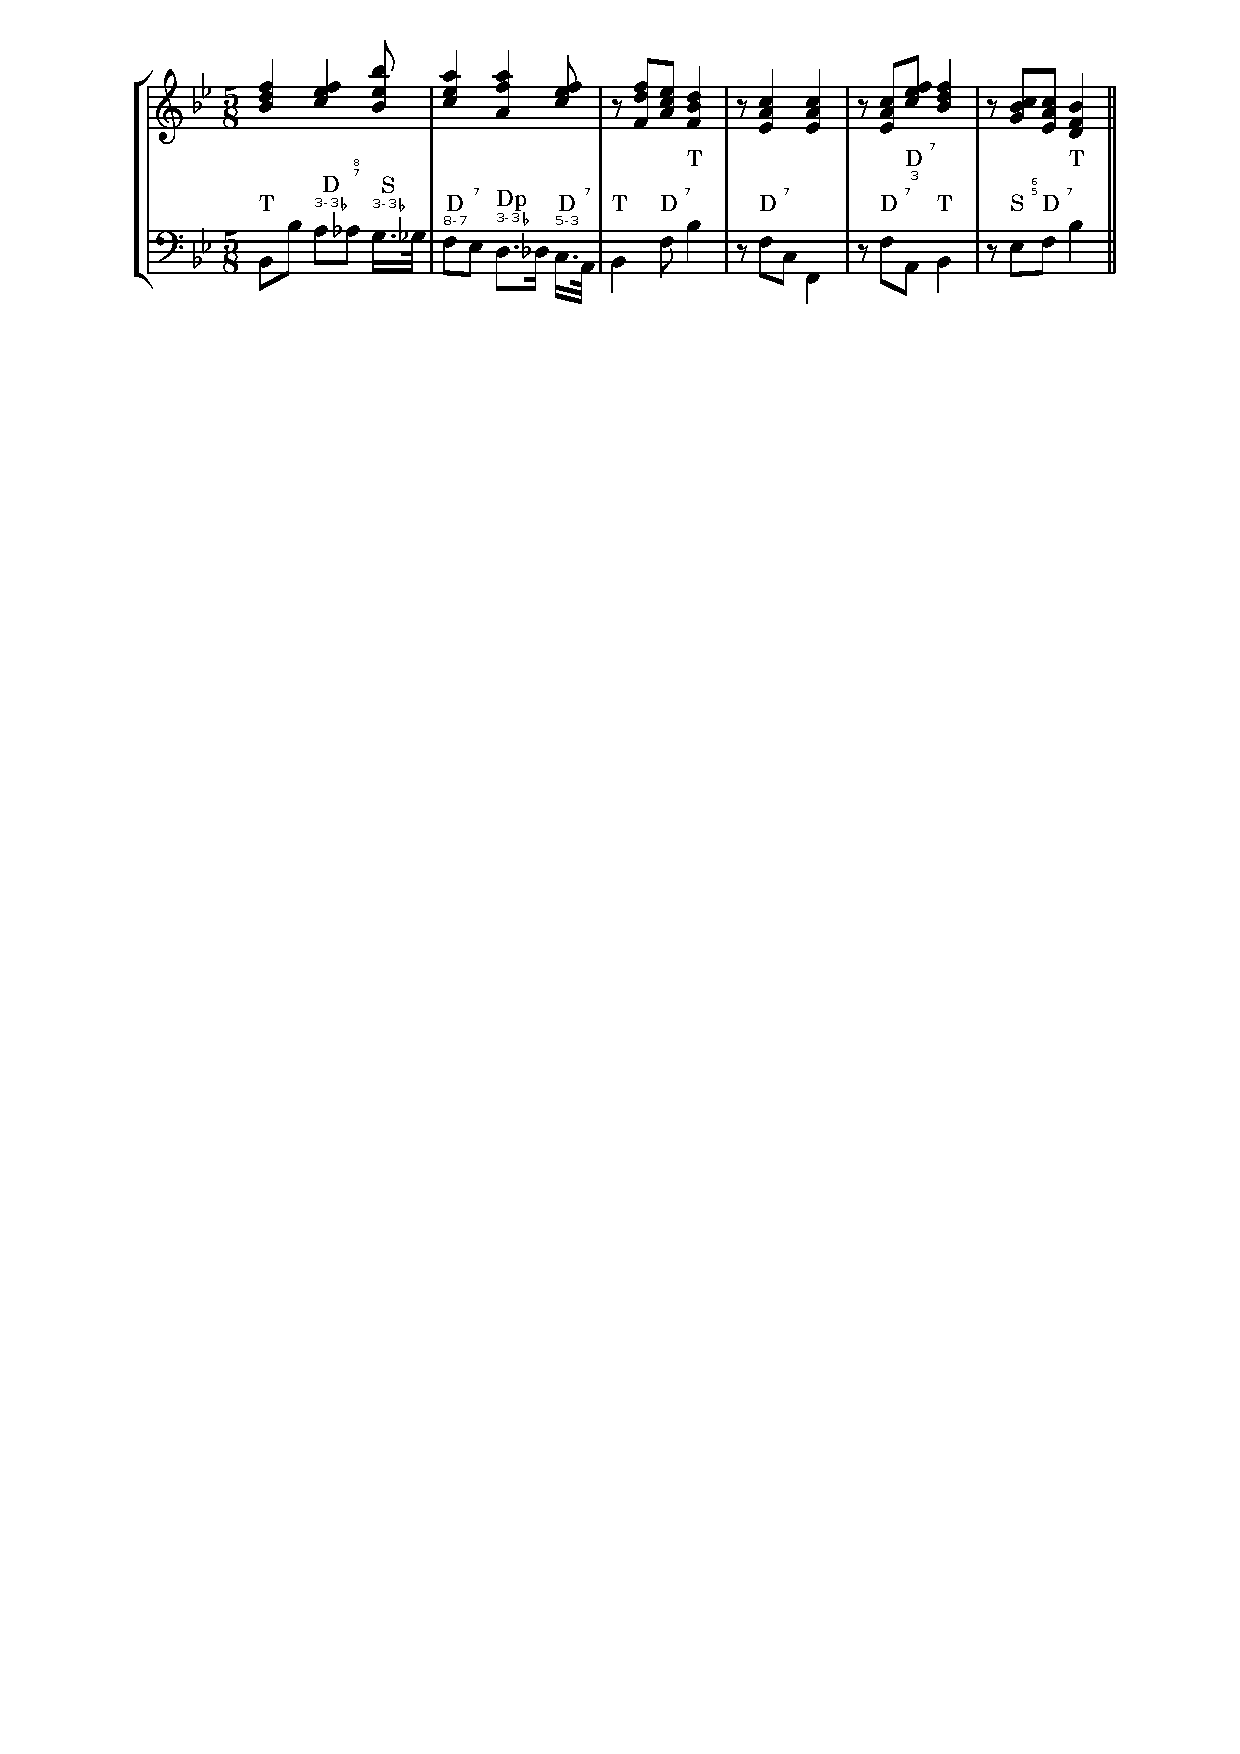
\includegraphics{pics/pmx/cadenca3}
\cad{III}{PMX}
\end{center}

Zu ihr gehört dieser Sourcecode:

\begin{verbatim}
%%% PREAMBLE: %%%%%%%%%%%%%%%%%%%%%%%%%%%%%%%%%%%%%%%%%%%%%%%%%%%%%%%
% nstaves | ninstr | mtrnuml  | mtrdenl | mtrnump | mtrdenp | npickup
     2        2         5          8         5         8         0
%  nkeys  | npages | nsystems | musicsize | fracident
     -2        0         3          16          .1
Bass
Diskant
bt
./
%%% BODY: %%%%%%%%%%%%%%%%%%%%%%%%%%%%%%%%%%%%%%%%%%%%%%%%%%%%%%%%%%% 
%%% HEADER: %%%%%%%%%%%%%%%%%%%%%%%%%%%%%%%%%%%%%%%%%%%%%%%%%%%%%%%%% 
\\font\ref=cmr10\def\zt#1#2{\zcharnote{#1}{\ref#2}}\def\bs{$\backslash$}\
%a smaller width than the line width
w130m
%%% MUSIC: %%%%%%%%%%%%%%%%%%%%%%%%%%%%%%%%%%%%%%%%%%%%%%%%%%%%%%%%%%%
%%% T1: %%%%%%%%%%%%%%%%%%%%%%%%%%%%%%%%%%%%%
[l b82 b8+ ] [l a8 a8f ] [l g1d g3 ] |/
\zt{-7}{T}\  b44u zd zf 
\zt{-7}{D7}\ cu ze zf 
\zt{-7}{S}\  b8-u ze zb+ |/
%%% T2: %%%%%%%%%%%%%%%%%%%%%%%%%%%%%%%%%%%%%
 [l f83 e83 ] [l d83d d13f ] [l c13d a32 ] |/
\zt{-7}{D7}\ c4-u ze za
\zt{-7}{Dp}\ a-u zd za+ 
\zt{-7}{D7}\ c8-u ze zf   |/
%%% T3: %%%%%%%%%%%%%%%%%%%%%%%%%%%%%%%%%%%%%
b42 f83 b43 |/
r8 \zt{-7}{T}\  [uh f85 zd zf-
   \zt{-7}{D7}\ e85 zc za ] 
   \zt{-7}{T}\  d4- zf zb |/
%%% T4: %%%%%%%%%%%%%%%%%%%%%%%%%%%%%%%%%%%%%
r8 f83 c83 f42 |/
r8 \zt{-7}{D7}\ e44 za zc e44 za zc |/
%%% T5: %%%%%%%%%%%%%%%%%%%%%%%%%%%%%%%%%%%%%
r8 [l f83 a8- ] b42l |/
r8 \zt{-7}{D7}\ [u c85 za ze c85 ze zf ] 
   \zt{-7}{T}\   b44u zf+ zd |/
%%% T6: %%%%%%%%%%%%%%%%%%%%%%%%%%%%%%%%%%%%%%
r8 [l e83 f8 ] b4l |/
r8 \zt{-7}{D7}\ [u c85 zb zg c85 za ze ] 
   \zt{-7}{T}\ b44u zf zd |/
%%%%%%%%%%%%%%%%%%%%%%%%%%%%%%%%%%%%%%%%%%% EOF
\end{verbatim}

Schon der erste Akkord aus der Musix\TeX-Variante
\begin{center}\texttt{\textbackslash{NOtes}
\textbackslash{Dqbl} I b \&
\textbackslash{zq}\{ik\}\textbackslash{qu}\{m\} \textbackslash{en}} \end{center}
reduziert\footnote{Um mal die reinen Notensymbole gegenüberzustellen, haben wir
diesmal die in beiden Varianten als \TeX-Code integrierten Analysesymbole n
weggelassen.} sich zum schlichteren
\begin{center}\texttt{[l b82 b8+ ] |/ b44u zd zf }\end{center}

\subsubsection{\ldots der Wermutstropfen \ldots}

Trotz der so euphorisch kolportierten Vorteile wächst sich \textit{PMX} bei
näherem Hinsehen für den Musikwissenschaftler jedoch zu einer Enttäuschung aus.
Gehen wir die Punkte der Reihe nach durch:

\paragraph{\small Inkompatibilitäten}$\;$ \\

Zunächst müssen wir 'gestehen', dass wir in diesem Kapitel unseres
'selbstreferentiellen' Dokumentes die Gegenüberstellung von Notentext und
generierendem Code nur scheinbar verwirklicht haben: Es gibt überhaupt keine
Möglichkeit, PMX-Code in \LaTeX-Code einzubetten und daraus dann -- sozusagen in
einem Rutsch -- eine PDF-Datei zu erzeugen.
Das liegt in erster Linie an der Arbeitsweise von \textit{PMX}\footnote{In zweiter
Linie liegt es an den Entwicklern von \textit{PMX}. Sie haben schlicht (noch) kein
korrespondierendes \LaTeX-Paket geschaffen. Technisch mag das herausfordernd
sein, unmöglich ist es nicht: Es wird ja schon gesagt, dass der von \textit{pmxab}
erzeugte Code eigentlich 'nur' auf die richtige Weise auskommentiert werden
müsse, damit er in der \texttt{\textbackslash{begin/end}\{music\}}-Umgebung
genutzt werden könne (\cite[vgl.][94]{Noack2013a}). Mithin sollte der Schritt zu
einer integrierten Lösung so groß nicht sein.}: Als Päprozessor nimmt das
entsprechende Tool \textit{pmxab} eine \textit{PMX}-Datei und erzeugt daraus eine
MusiX\TeX-Datei. Diese MusiX\TeX-Datei ist von ihrem Dialekt her aber eine
vollständige MusiX\TeX-Datei und kein inkludierbares Code-Snippet, das 1:1 in die
\LaTeX-Umgebung
\texttt{\textbackslash{begin}\{music\} \ldots \textbackslash{end}\{music\}}
eingebettet werden könnte. Entsprechende Versuche müssen scheitern.


\begin{verbbox}[\footnotesize]
.pmx.eps:
  @ make \$< `basename \$< .pmx`.tex
  @ musixtex -g `basename \$< .pmx`.tex
  @ ps2eps `basename \$< .pmx`.ps
.pmx.tex:
   @ pmxab \$<
\end{verbbox}

\label{PmxGraphics} Die eine, 'direkte' Lösung für dieses Problem besteht darin,
zuerst -- ganz \LaTeX-unabhängig -- aus der \textit{PMX}-Datei eine Graphik zu
erzeugen und diese anschließend in die \LaTeX-Datei einzubinden\footcite[Vgl.
dazu auch][94]{Noack2013a}:

\begin{itemize}
  \item Dazu ruft man für eine \textit{PMX}-Datei zunächst den
  \textit{PMX}-Präprozessor auf (z.B. \texttt{pmxab candeza1.pmx}), um die
  korrespondierende MusiX\TeX-Datei \texttt{candeza1.tex} zu genieren.
  \item Das Resultat übergibt man dann dem \textit{MusiX\TeX}-Tool als Input, und
  zwar mit der Option \textit{-g}: (\texttt{musixtex -g candeza1.tex}). So wird
  nicht eine \textit{PDF}-Datei erzeugt, sondern die Postscriptdatei
  \texttt{candeza1.ps}.
  \item Danach lässt man diese Postscriptdatei in eine 
  Encapsulated-Postscript-Datei umwandeln (\texttt{ps2eps
  candeza1.ps})\footnote{Eine make-basierte
  Automatisierung dieser Schritte enthielte als Kern wohl dies:\vspace{0.2em}\\
  \theverbbox\ \vspace{0.2em}\\
  \cite[Vgl. dazu][\nopage Makefile aus dem Verzeichnis 'pmx']{Reincke2019a}.}
  \item Und ganz zuletzt fügt man an der Stelle der \LaTeX-Datei, wo die
  \textit{eps}-Graphik erscheinen soll, den \LaTeX-Befehl 
  \texttt{\textbackslash{includegraphics}\{candeza1.eps\}}
  ein\footnote{Hier muss man beachten, an der Stelle, von wo aus man die
  \textit{eps}-Datei einlesen will, nicht (versehentlich) auch eine 'gleichnamige'
  \textit{pdf}-Datei abgelegt zu haben. In diesem Fall lädt
  \texttt{includegraphix} nämlich letztere. Und das wird im \LaTeX-Dokument zu
  unerwarteten Seitenumbrüchen führen, nach deren Ursache man u.U. lange sucht.
  }.
\end{itemize}

Diese Umstände müssen -- wenigstens den Musikwissenschaftler -- enttäuschen:
Wenn man zuletzt doch eine Graphik einbindet, die man mit einem externen Tool
erstellt hat, warum sollte man sich dann die Mühe antun, zwecks Erstellung einer
Graphik zuerst \textit{PMX} zu lernen, wo es doch so viele gute Notenprogramme
gibt, die ihre Daten auch als Postscript- oder PDF-Datei
exportieren?\footnote{Zu Erinnerung: \textit{ABC} geht implizit genauso vor.
Insofern träfe dieses Argument eben auch \textit{ABC}. Allerdings punktet
\textit{ABC} durch seine vielen Konverter und Tools und durch seine lange
Tradition.} Das könnte doch nur dann sinnvoll sein, wenn man wenigstens auf die
gestalterischen Vorzüge und Freiheiten von MusiX\TeX\ zugreifen könnte. Aber
nicht einmal das ist ja der Fall -- wie wir gleich sehen werden.

Zunächst müssen wir aber der Wahrheit Genüge tun und darauf hinweisen, dass der
Autor des \textit{PMX}-Tutorials sehr wohl um die Irritationen in Sachen \textit{PMX
/ MusiX\TeX}\ und \textit{\LaTeX}\ weiß, ja mehr noch, dass er sie auch nicht
verschweigt: Beide Ansätze würden  -- obwohl sie auf \TeX\ beruhen --
konkurrierend und überschneidend das Layout gestalten und viel Spezialbefehle
zueinander inkompatibel definieren\footcite[vgl.][93]{Noack2013a}. Und so kommt
er zu dem Schluss:

\begin{quote}\textit{\enquote{While with modern implementations of ressources
are no longer a serious problem, the incompatibility problems are, and their
resolution would be a major programming task. So there have, to this day, not
been any serious efforts to provide a truly merged version of \LaTeX\ with
PMX.}\footnote{\cite[vgl.][93f]{Noack2013a}. Man muss an dieser Stelle auch
im Kopf behalten, dass PMX nicht für die Nutzung in \LaTeX\ entwickelt worden ist.
Es ging den Entwicklern darum, besser und einfacher qualitativ hochwertige
Notenblätter zu erzeugen. Und für diesen Zweck ist die Lösung \textit{PMX
/ MusiX\TeX} sehr wohl geeignet. Nur ist die Gestaltung solcher Blätter meist nicht
Aufgabe von Musikwissenschaftlern.}
}\end{quote}

\paragraph{\small Unzulänglichkeiten}$\;$ \\

Die erste kleinere Unzulänglichkeit betrifft das Erscheinungsbild: Die
Kadenz-III in der \textit{PMX}-Variante\footnote{$\rightarrow$ S.
\pageref{\cadlab{III}{PMX}}} wirkt optisch weniger klar als die
\textit{MusiX\TeX}-Variante\footnote{$\rightarrow$ S.
\pageref{\cadlab{III}{MusiXTeX}}}. Dies liegt am 5/8-Takt. Der kann in eine 3er-
und eine 2er Hälfte oder in eine 2er und eine 3er Hälfte aufgeteilt werden. Und
das 3. Achtel der 3er-Hälfte kann auftaktisch gemeint sein. Die Entscheidungen,
die \textit{PMX} -- sozusagen nach Schema F -- automatisch trifft, können solchen
fallweisen Feinheiten natürlich nicht gerecht werden\footnote{Gelegentlich wird
man diese allerdings auch für reine Geschmacksfragen halten dürfen.}.

Die zweite Unzulänglichkeit betrifft die Methode, wie die Analysesymbole in den
\textit{PMX}-Code eingettet werden: \textit{PMX} bietet zwar die Möglichkeit, Stücke
auf \textit{PMX}-Level textuell zu kennzeichnen oder Texte über oder unter den
Systemen einzufügen\footcite[vgl.][61f]{Noack2013a}. Wenn es aber -- wie bei der
Musikwissenschaft notwendig -- darum geht, Symbole und Texte graphisch variabel
einzufügen, dann muss der \textit{PMX}-User auf \enquote{Inline \TeX\ commands}
zurückgreifen, also unter den \LaTeX-Level auf den \TeX-Level
'zurückfallen'\footcite[vgl.][76f]{Noack2013a}: die Nutzung einer vereinfachten
\textit{PMX}-Syntax wird dann um den Preis einer komplizierten Eingabe von
\TeX-Syntagmen erkauft\footnote{Weil \TeX\ 'zu' kompliziert war, wurde \LaTeX\
'erfunden'; und weil \textit{PMX} mit Text 'zu' kompliziert war, entstand
\textit{M-Tx} (\cite[vgl.][\nopage wp]{CtanMtx2018a}) -- einschließlich eines
Handbuches (\cite[vgl.][3ff]{Laurie2017a})}.

Wirklich unzulänglich ist dabei jedoch das, \textit{was} eingebettet werden kann.
Was schon bei den ABC-Lösungen galt\footnote{$\rightarrow$ S.
\pageref{AppraisalABC}}, gilt auch hier: Aus der \LaTeX-Welt können weder hoch-
und/oder tiefgestellte Kleinsymbole oder Sonderzeichen eingefügt werden, noch
die Alterationszeichen $\sharp$, $\flat$ oder $\natural$ aus den Sonderzeichen -
ganz zu schweigen von der Einbettung jener ausgefeilten Konstrukte, die das
\textit{harmony}-Paket zur Verfügung stellt. Denn das Konvertierungstool
\textit{pmxab}, das \textit{MusiX\TeX}-Code aus \textit{PMX}-Code ableitet, arbeitet
ja noch außerhalb von \TeX. Und das Konvertierungsttool \textit{musixtex}
versteht 'nur' \textit{Musix\TeX}-Code, nicht aber \LaTeX-Syntagmen.

\subsubsection{\ldots und die kleine Lösung: Kadenz II}

Trotz all dieser Nicklichkeiten kann es für den Musikwissenschaftler
gelegentlich sehr wohl Sinn machen, im Kontext einer \LaTeX-Arbeit\footnote{mit
inkludiertem MusiX\TeX-Package} auf \textit{PMX} zurückzugreifen: Wenn es nämlich
gilt, viele längere Musikbeispiele zu verwenden, wird das manuelle Tippen des
MusiX\TeX-Codes zu einer langwierigen, fehlerträchtigen Angelegenheit werden.

Eine Lösung dafür bestünde darin, zuerst den reinen Notentext mit \textit{PMX} zu
erstellen und dann mit \textit{pmxab} in MusiX\TeX-Code umzuwandeln. Danach griffe
man auf die Option zurück, -- wie im Tutorial als Möglichkeit angedeutet --
\enquote{manuell} bestimmte Zeilen des automatisch generierten Codes
auszukommentieren und so etwas zu erzeugen, was tatsächlich in die
\verb|\begin{music}...\end{music}|-\LaTeX-Umgebung kopiert werden
kann\footcite[vgl.][94]{Noack2013a}. Dieses Verfahren wollen wir noch kurz
vorführen:

Wir wissen ja schon, dass wir die Symbole der Harmonieanalyse, die wir auf
\textit{PMX}-Level erstellen könnten, bei einer Einbettung in einen \LaTeX-Code
werden nicht verwenden können, eben weil es ja keine \LaTeX-Konstrukte sind,
sondern \TeX-Syntagmen. Deshalb notieren wir diesmal auf \textit{PMX}-Level nur
den Notentext. Das 'reine' PMX/MusiX\TeX-Verfahren\footnote{PMX-Code $\rightarrow$
\texttt{pmxab} $\rightarrow$ Musix\TeX-Code $\rightarrow$ \texttt{musictex -g} 
$\rightarrow$ PS-Code  $\rightarrow$ \texttt{ps2eps} $\rightarrow$ EPS-Graphik }
würde daraus die folgende Graphik erzeugen:

\begin{center}
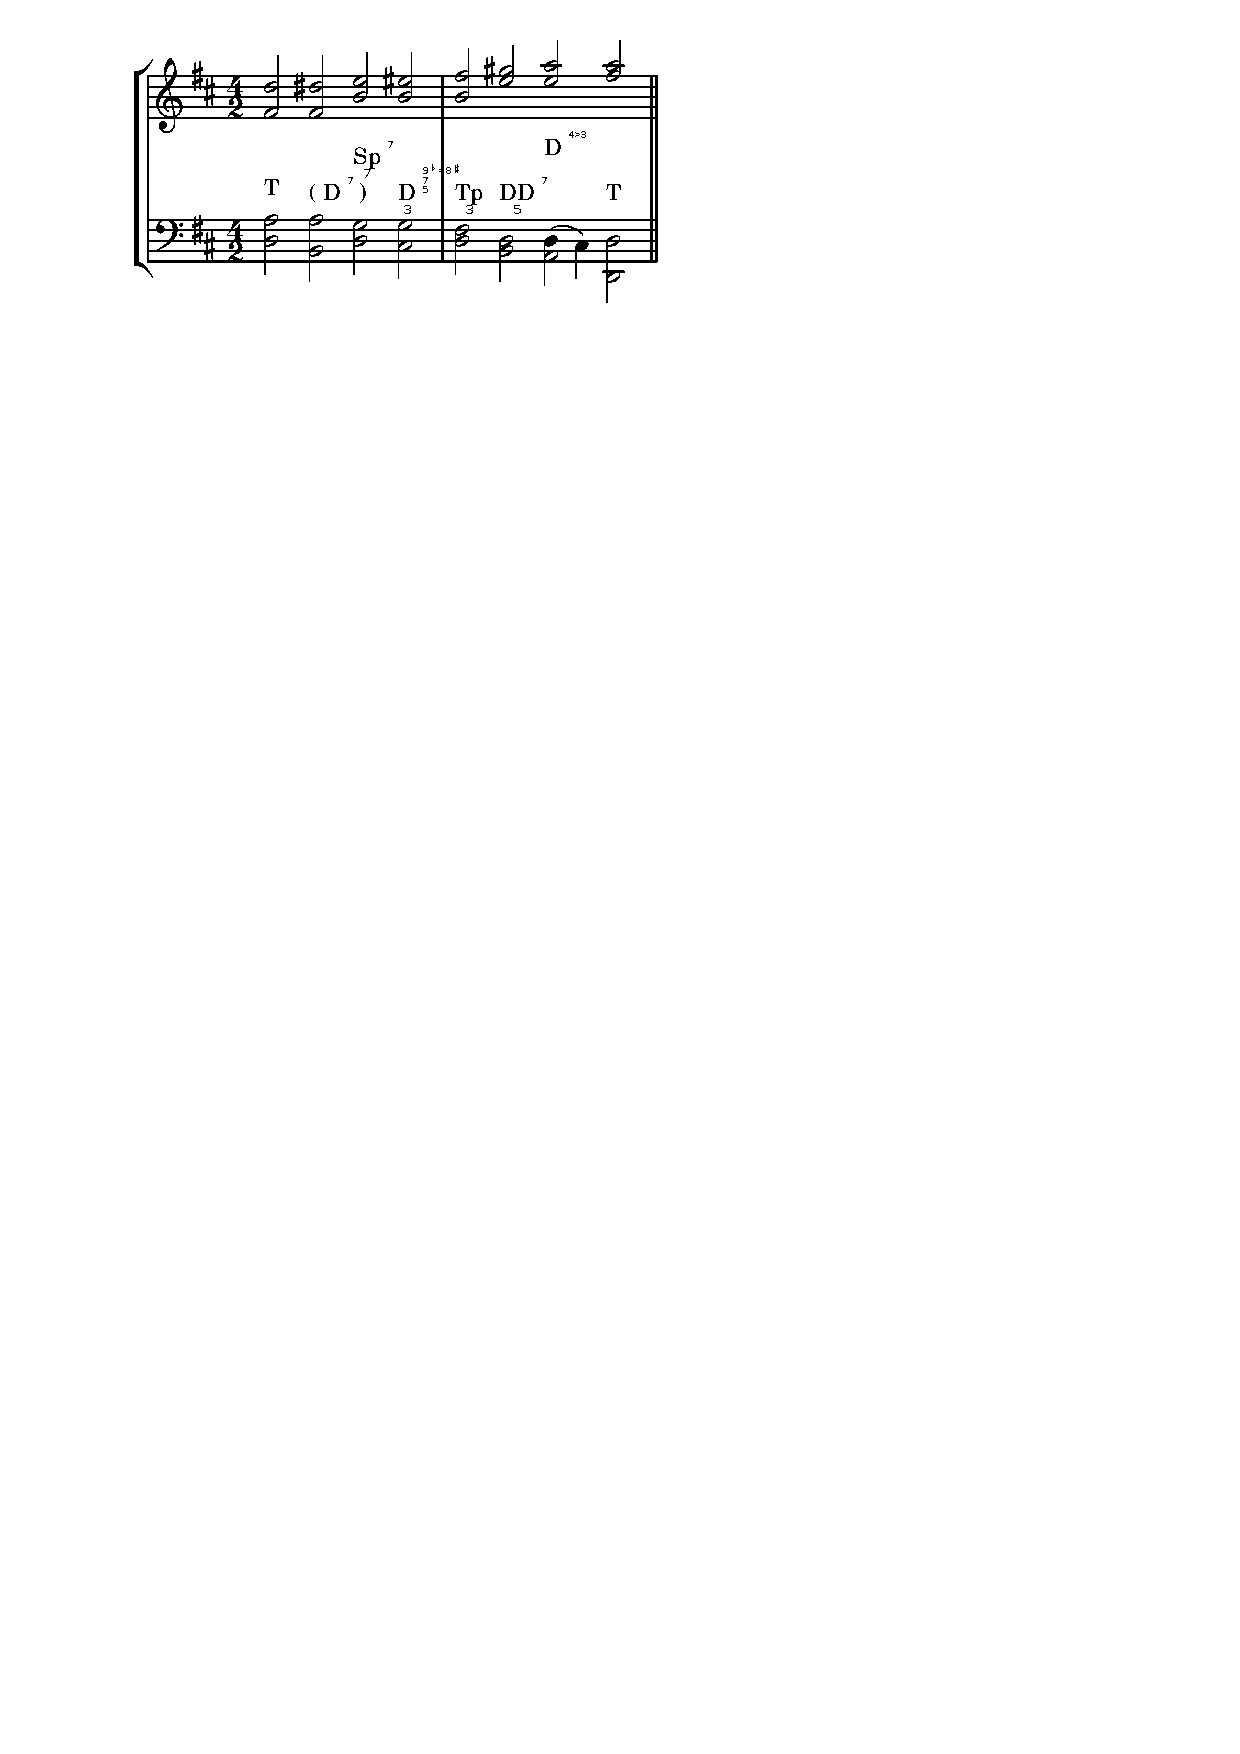
\includegraphics{pics/pmx/cadenca2}
\cad{II}{PMX}
\end{center}

Ausgegangen wird dabei von folgendem \textit{PMX}-Code:

\begin{verbatim}
% PREAMBLE %%%%%%%%%%%%%%%%%%%%%%%%%%%%%%%%%%%%%%%%%%%%%%%%%%%%%%%%%%
% nstaves | ninstr | mtrnuml  | mtrdenl | mtrnump | mtrdenp | npickup
     2        1         4          2         4         2         0
%  nkeys  | npages | nsystems | musicsize | fracident
     2        0         3          16          .1
Piano
bt
./
% BODY: %%%%%%%%%%%%%%%%%%%%%%%%%%%%%%%%%%%%%%%%%%%%%%%%%%%%%%%%%%%%%
% HEADER: %%%%%%%%%%%%%%%%%%%%%%%%%%%%%%%%%%%%%%%%
%a smaller width than the line width
w130m
% MUSIC: %%%%%%%%%%%%%%%%%%%%%%%%%%%%%%%%%%%%%%%%%
% T:1-1     T:1-2    T:1-3                T:1-4
  d23l za+  b-l za+  d-l zg              c-l zg+ |/
  f24u zd+  f-u zd+s  bu  ze              bu zes |/
% %%%%%%%%%%%%%%%%%%%%%%%%%%%%%%%%%%%%%%%%%%%%%%%%%
% T:2-1     T:2-2    T:2-3                T:2-4
  d23l zf  b-l  zd   (u d4 za2 c4 za2 )   d2-l zd+  /
  b24u zf+  e  zgs   e  za                f  za |/
% %%%%%%%%%%%%%%%%%%%%%%%%%%%%%%%%%%%%%%%%%%%%%  EOF 
\end{verbatim}

Lässt man diesen \textit{PMX}-Code von \texttt{pmxab} verarbeiten, entsteht ein
Musix\TeX-Code, bei dem man, will man ihn erfolgreich in eine
Musix\TeX-in-\LaTeX-Umgebung \verb|\begin{music}| ... \verb|\\end{music}|
einbetten, noch  einige Zeilen auskommentieren und einige Werte ändern muss:

\begin{verbatim}
\begin{music}
%%ignore:%% \input musixtex
%%ignore:%% \input pmx
%%ignore:%% \setmaxslurs{24}\setmaxinstruments{24}%
\normalmusicsize %%% instead of: %%% \smallmusicsize%
%%ignore:%% \nopagenumbers
%%ignore:%% \tracingstats=2\relax
%%ignore:%% \hsize=369pt
%%ignore:%% \vsize740pt
\def\nbinstruments{1}
\setstaffs12
\setclef1{60}
\setname1{Piano}
\generalsignature{ 2}%
\generalmeter{\meterfrac{4}{2}}%
\parindent 4em %%% instead of %%% 37pt
%%ignore:%% \elemskip1pt\afterruleskip1.000pt\beforeruleskip0pt\relax
%%ignore:%% \stafftopmarg0pt\staffbotmarg5\Interligne\interstaff{10}\relax
%%ignore:%% \readmod{cadenca2}
%%ignore:%% \startmuflex
\startpiece
%%ignore:%% \addspace
%%ignore:%% \afterruleskip%
%%ignore:%% \znotes|\zcharnote{16}{\titles{2.0}{}{0}{}{0}{}{0}}\en%
% Bar count 1
\pnotes{4.00}\zh{''A}\hl{`D}\zh{'A}\hl{`B}\zh G\hl D\zh G\hl C|\zh{'d}%
\hu{`f}\bigsh{'d}\zh d\hu{`f}\zh{'e}\hu b\bigsh e\zh e\hu b\en%
% Bar count 2
\xbar
\pnotes{4.00}\zh{'F}\hl D\zh D\hl B|\zh{'f}\hu b\bigsh g\zh g\hl e\en%
\pnotes{2.83}\zq A\qu D \zq A\qu C|\zh{''a}\hl{`e}%
%%ignore: \isu0{'D}{.8} \tslur0A
\en%
\pnotes{4.00}\zh{'D}\hl{`D}|\zh{''a}\hl{`f}\en%
\Endpiece
%%ignore:%% \vfill\eject\endmuflex
%%ignore:%% \bye
\end{music}%
\end{verbatim}

Vor einer erfolgreichen Nutzung diese Codes muss man in seinem \LaTeX-Header
auch noch die Regel \verb|\newcommand{\pnotes}[1]{\notes}| formuliert haben,
damit aus der Einbettung auf \LaTeX/MusiX\TeX-Ebene -- also ohne Einbindung
einer externen Graphik -- das folgende Bild  entsteht:

\vspace{0.7cm}
\begin{music}
%%ignore:%% \input musixtex
%%ignore:%% \input pmx
%%ignore:%% \setmaxslurs{24}\setmaxinstruments{24}%
\normalmusicsize %%% instead of: %%% \smallmusicsize%
%%ignore:%% \nopagenumbers
%%ignore:%% \tracingstats=2\relax
%%ignore:%% \hsize=369pt
%%ignore:%% \vsize740pt
\def\nbinstruments{1}
\setstaffs12
\setclef1{60}
\setname1{Piano}
\generalsignature{ 2}%
\generalmeter{\meterfrac{4}{2}}%
\parindent 4em %%% instead of %%% 37pt
%%ignore:%% \elemskip1pt\afterruleskip1.000pt\beforeruleskip0pt\relax
%%ignore:%% \stafftopmarg0pt\staffbotmarg5\Interligne\interstaff{10}\relax
%%ignore:%% \readmod{cadenca2}
%%ignore:%% \startmuflex
\startpiece
%%ignore:%% \addspace
%%ignore:%% \afterruleskip%
%%ignore:%% \znotes|\zcharnote{16}{\titles{2.0}{}{0}{}{0}{}{0}}\en%
% Bar count 1
\pnotes{4.00}\zh{''A}\hl{`D}\zh{'A}\hl{`B}\zh G\hl D\zh G\hl C|\zh{'d}%
\hu{`f}\bigsh{'d}\zh d\hu{`f}\zh{'e}\hu b\bigsh e\zh e\hu b\en%
% Bar count 2
\xbar
\pnotes{4.00}\zh{'F}\hl D\zh D\hl B|\zh{'f}\hu b\bigsh g\zh g\hl e\en%
\pnotes{2.83}\zq A\qu D \zq A\qu C|\zh{''a}\hl{`e}%
%%ignore: \isu0{'D}{.8} \tslur0A
\en%
\pnotes{4.00}\zh{'D}\hl{`D}|\zh{''a}\hl{`f}\en%
\Endpiece
%%ignore:%% \vfill\eject\endmuflex
%%ignore:%% \bye
\end{music}%
\cad{II}{PMX+MusiXTeX-in-LaTeX}
\vspace{0.7cm}

An dieser Version erkennt man jedoch auch, dass die Vorstellung, man brauche
bloß mal eben Zeilen auszukommentieren, der Sachlage nicht gerecht wird: Damit
obiger Code überhaupt kompilierbar wurde, mussten wir die Vorhaltsklammer im
Bass aus dem Code herausnehmen, was dort unmittelbar zu einer ungewollten
Oktavierung führte. Tatsächlich wird man -- falls man den MusiX\TeX-Code in
seinen \LaTeX-Code einfügen will, den \texttt{pmxab} aus der \textit{pmx}-Datei
erzeugt -- ein wenig 'Tuning'-Zeit einplanen müssen. Geht man diesen Weg, kann
man nun allerdings auch die \LaTeX-basierten Elemente einer Harmonieanalyse
darin verwenden. Man hat also in der Tat die gestalterische Freiheit auf
\LaTeX-MusiX\TeX-Level gewonnen, ohne den komplexen und komplizierten
MusiX\TeX-Code als Ganzes selbst entworfen haben zu müssen. Die Grundarbeit
erledigt man auf \textit{PMX}-Level, die Feinheiten fügt man manuell ein:

\vspace{0.7cm}
\begin{music}%
\normalmusicsize %%% instead of: %%% \smallmusicsize%
\def\nbinstruments{1}
\setstaffs12
\setclef1{60}
\setname1{Piano}
\generalsignature{ 2}%
\generalmeter{\meterfrac{4}{2}}%
\parindent 4em %%% instead of %%% 37pt
\startpiece
% Bar count 1
\notes
  \zmidstaff{\HH.T.....}\zh{''A}\hl{`D}%
  \zmidstaff{(\HH.D..7...)}\zh{'A}\hl{`B}%
  \zmidstaff{\HH.Sp.7...7.}\zh G\hl D
  \zmidstaff{\HH.\Dohne.3.$\flat$9=$\sharp$8.7.5.}\zh G\hl C |%
  \zh{'d}\hu{`f}\bigsh{'d}\zh d\hu{`f}%
  \zh{'e}\hu b\bigsh{e}\zh e\hu b%
\en%
% Bar count 2
\xbar
\notes
  \zmidstaff{\HH.Tp.3....}\zh{'F}\hl D%
  \zmidstaff{\HH.\DD.5...7.}\zh D\hl B |%
  \zh{'f}\hu b\bigsh g%
  \zh g\hl e%
\en%
\notes
  \zmidstaff{\HH.D....4-3.}%
  \zh{H}\isluru{0}{K}\qu{K}\tslur{0}{J}\qu{J}|%
  \zh{''a}\hl{`e}%
\en%
\notes
  \zmidstaff{\HH.T.....}\zh{'D}\hl{`D}  |%
  \zh{''a}\hl{`f}%
\en%
\Endpiece
\end{music}%
\cad{II}{PMX+MusiXTeX-in-LaTeX++}
\vspace{0.7cm}
 
Hilfreich sind dabei -- zugegebenermaßen -- Geduld, ein geschulter Blick und der
Wille zum Codeclearing:

\begin{verbatim}
\begin{music}%
\normalmusicsize %%% instead of: %%% \smallmusicsize%
\def\nbinstruments{1}
\setstaffs12
\setclef1{60}
\setname1{Piano}
\generalsignature{ 2}%
\generalmeter{\meterfrac{4}{2}}%
\parindent 4em %%% instead of %%% 37pt
\startpiece
% Bar count 1
\notes
  \zmidstaff{\HH.T.....}\zh{''A}\hl{`D}%
  \zmidstaff{(\HH.D..7...)}\zh{'A}\hl{`B}%
  \zmidstaff{\HH.Sp.7...7.}\zh G\hl D
  \zmidstaff{\HH.\Dohne.3.$\flat$9=$\sharp$8.7.5.}\zh G\hl C |%
  \zh{'d}\hu{`f}\bigsh{'d}\zh d\hu{`f}%
  \zh{'e}\hu b\bigsh{e}\zh e\hu b%
\en%
% Bar count 2
\xbar
\notes
  \zmidstaff{\HH.Tp.3....}\zh{'F}\hl D%
  \zmidstaff{\HH.\DD.5...7.}\zh D\hl B |%
  \zh{'f}\hu b\bigsh g%
  \zh g\hl e%
\en%
\notes
  \zmidstaff{\HH.D....4-3.}%
  \zh{H}\isluru{0}{K}\qu{K}\tslur{0}{J}\qu{J}|%
  \zh{''a}\hl{`e}%
\en%
\notes
  \zmidstaff{\HH.T.....}\zh{'D}\hl{`D}  |%
  \zh{''a}\hl{`f}%
\en%
\Endpiece
\end{music}
\end{verbatim}


% this is only inserted to eject fault messages in texlipse
% \bibliography{../bib/literature}


% mycsrf 'for beeing included' snippet template
%
% (c) Karsten Reincke, Frankfurt a.M. 2012, ff.
%
% This text is licensed under the Creative Commons Attribution 3.0 Germany
% License (http://creativecommons.org/licenses/by/3.0/de/): Feel free to share
% (to copy, distribute and transmit) or to remix (to adapt) it, if you respect
% how you must attribute the work in the manner specified by the author(s):
% \newline
% In an internet based reuse please link the reused parts to mycsrf.fodina.de
% and mention the original author Karsten Reincke in a suitable manner. In a
% paper-like reuse please insert a short hint to mycsrf.fodina.de and to the
% original author, Karsten Reincke, into your preface. For normal quotations
% please use the scientific standard to cite
%


%% use all entries of the bibliography

\subsection{Lilypond: so schön, wie vielversprechend ($\bigstar\bigstar\bigstar\bigstar\bigstar$)}

\parpic(2cm,1.4cm)[r][t]{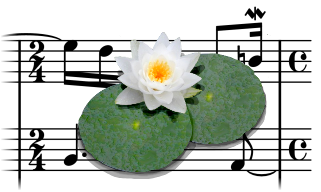
\includegraphics[width=2cm]{logos/lilypond-300dpi.png}}
\textit{LilyPond} möchte guten \enquote{Notensatz für jedermann} anbieten: Als
elektronisches \enquote{Notensatzsystem} -- so das Entwicklungsteam -- wolle es
\enquote{[\ldots] Notendruck in (bester) Qualität} ermöglichen, mithin
\enquote{[\ldots] die Ästhetik handgestochenen traditionellen Notensatzes mit
computergesetzten Noten [\ldots] erreichen}.\footnote{\cite[vgl.][\nopage
wp]{LilyPond2018a}. Lizensiert ist \acc{LiyPond} unter der GPL $\rightarrow$
\href{http://lilypond.org/gpl.html}{http://lilypond.org/gpl.html}, einer
anerkannten Open-Source-Lizenz ($\rightarrow$
\href{https://opensource.org/licenses/GPL-2.0}
{https://opensource.org/licenses/GPL-2.0}). } In einem besonderen Artikel haben
die LilyPond-Entwickler dargestellt, was das systemisch
bedeutet\footcite[vgl.][5ff]{LilyPond2018d} und welchen Konsequenzen sich daraus
für ein Notensatzprogramm ergeben.\footcite[vgl.][8ff]{LilyPond2018d} Der daraus
erwachsende Anspruch ist hoch:

\begin{quote}\textit{\enquote{LilyPond wurde geschaffen, um die Probleme zu
lösen, die wir in existierenden Programmen gefunden haben und um schöne Noten zu
schaffen, die die besten handgestochenen Partituren
imitieren.}\footcite[vgl.][2]{LilyPond2018d} }
\end{quote}

Wer die entsprechenden Techniken erfolgreich anwenden will, kann auf ein einfach
strukturiertes Lerntutorial\footcite[vgl.][20ff]{LilyPond2018b} und ein kürzeres
Nutzungshandbuch\footcite[vgl.][1ff]{LilyPond2018e} zurückgreifen. Letztlich
wird er sich allerdings auch das umfangreiche
Notationshandbuch\footcite[vgl.][1ff]{LilyPond2018c} bereitlegen wollen.

Wie die bisher diskutierten Systeme erwartet \textit{LilyPond}, dass man Code
schreibt, keine Noten: Hier wie da ist der Texteditor das bevorzugte Werkzeug,
um Musik im entsprechenden 'Dialekt' zu notieren. Trotzdem gibt es Unterschiede,
die über die bloße Syntax hinausgehen:

Die wichtigste Eigenart dürfte sein, dass Lilypond konsequent zwischen Musik und
Druck unterscheidet: Wer in D-Dur ein \textit{fis} einfügen möchte, kann sich
hier nicht auf die zu Beginn spezifizierte Tonart 'berufen', er muss trotzdem
\texttt{fis} tippen, nicht \texttt{f}, und zwar an jeder Stelle, wo er
\textit{fis} meint. Diese Abkehr von der musikalischen Tradition hat einen
gewichtigen Vorteil: Lilypond kann bei Alterationen die nötigen Vorzeichen
automatisch setzen. In \textit{g-moll} erhält die Note \textit{f} bei
eingegebenem \texttt{fis} automatisch ein Kreuz, in D-Dur
nicht.\footnote{\cite[vgl.][21]{LilyPond2018b}. In der Konsequenz wird man sich
allerdings auch an -- wenigstens für Deutsche -- überraschende 'Töne' wie
\texttt{bes}, \texttt{beses} oder \texttt{bis} gewöhnen müssen.}

Die augenfälligste Besonderheit dürfte jedoch sein, dass \textit{LilyPond} seine
Elemente konsequent in einer 1:n-Beziehung anordnet: Das Notenheft besteht aus
einem oder mehreren Stücken, das Stück besteht aus einem oder mehreren
Notensystemen, ein Notensystem besteht aus einer oder mehrerer Stimmen, die
Stimme kann solistisch oder akkordisch sein. Das Datenmodell ist mithin als
Baum\footcite[vgl.][\nopage wp.]{WpedBaum2019a} ausgelegt. Und syntaktisch haben
die Ebenen je eigene Markanten. Das macht das Lesen und Verstehen von
\textit{LilyPond}-Code auf Dauer einfacher, es entsteht ein klarerer
Sourcetext.\footcite[vgl.][40ff]{LilyPond2018b}

Systemisch gesehen hat LilyPond (heute) nichts (mehr) \LaTeX\ , MusiX\TeX\ oder
\TeX\ zu tun: es nutzt seine eigene Eingabesprache und seine eigene Maschine zum
Erzeugen des Notenbildes: Als \enquote{Standardausgabeformat} -- heißt es --
seien \textit{PDF}\footnote{Portable Document Format} und
\textit{PS}\footnote{Postscript} gesetzt; außerdem könnten
\textit{SVG\footnote{Scalable Vector Graphics}-}, \textit{EPS\footnote{Encapsulated
PostScript}-} und \textit{PNG\footnote{Portable Network Graphics}-}Dateien erzeugt
werden.\footcite[vgl.][481]{LilyPond2018c}

\subsubsection{Technische Voraussetzungen}

\textit{LilyPond} sagt selbst, dass man Notenbeispiele in Form von Graphiken auch
manuell in den \LaTeX-Text einfügen könne, einfach indem man -- zuerst und
unabhängig von \LaTeX\ -- die Graphiken mit \texttt{lilypond} erzeuge und sie
danach mit \LaTeX-Mitteln einbinde.\footcite[vgl.][20]{LilyPond2018e} Bei vielen
Notenbeispielen kann das allerdings aufwendig werden, insbesondere, wenn man
manuell die Länge der Notenzeilen und die Graphikbreite auf die gewünschte
Zeilenlänge des Dokumentes ausrichten muss.

Deshalb bietet \textit{LilyPond} nicht nur das Tool \texttt{lilypond} zur
Erzeugung ganzer Notenblätter in den genannten Formaten an\footnote{samt aller
anderen Outputformate wie \textit{midi} u.Ä.m.}, sondern auch das Tool
\texttt{lilypond-book}: dieses \enquote{automatisiert} die manuelle Integration,
indem es die \enquote{[\ldots] Musik-Schnipsel aus Ihrem Dokument (extrahiert),
[\ldots] \texttt{lilypond} (aufruft) und [\ldots] die resultierenden Bilder in
Ihr Dokument (einfügt)}, wobei es \enquote{[\ldots] die Länge der Zeilen und die
Schriftgröße dabei [automatisch] (dem) Dokument
(anpasst)}.\footcite[vgl.][20]{LilyPond2018e}

Daraus folgt sofort, dass man auch hier einiges vorzubereiten hat, wenn man
\textit{LilyPond} erfolgreich verwenden will:

$\RHD$ Zunächst muss man -- ganz unabhängig von \LaTeX\ -- \textit{LilyPond}
installieren\footnote{Unter Ubuntu: \texttt{sudo apt-get lilypond
lilypond-data}}. Dieses Paket stellt dann auch \texttt{lilypond-book} bereit.
  
$\RHD$ Im Gegensatz zu \textit{ABC} oder \textit{MusiX\TeX} braucht \acc{LilyPond}
nicht in der \LaTeX-Präambel aktiviert zu werden. Denn \texttt{lilypond-book} muss
ja immer zuerst und unabhängig von \LaTeX\ aufgerufen werden: Es generiert erst den
eigentlichen \LaTeX-Code, der dann keine \textit{LilyPond}-Sektionen mehr
enthält. Also kann man -- direkt nach der Installation -- den
\textit{LilyPond}-Quelltext eines jeden Notenbeispiels in je einer eigenen
(virtuellen) Umgebung \verb|\begin{lilypond}...\end{lilypond}| editieren.
Virtuell sind diese Umgebungen insofern, als \LaTeX\ ja nichts von
\textit{LilyPond} weiß.

$\RHD$ Schließlich muss man noch organisieren, dass den eigentlichen
\LaTeX-Durchgängen zur Generierung der PDFs ein \texttt{lilypond-book}-Aufruf
vorausgeht. Das kann wieder in einem Makefile organisiert werden.

Leider steckt der Teufel dabei -- wie so oft -- im Detail: 

\label{LilyPondGraphics}\texttt{lilypond-book} nimmt eine -- wie wir jetzt
wissen -- gewissermaßen 'unechte' \LaTeX-Datei, die noch
\textit{lilypond}-Sektionen enthält, und erzeugt die entsprechenden Graphiken,
bevor es die \textit{lilypond}-Sektionen durch die korrespondierenden
'include-Graphik'-Befehle auf \LaTeX-Ebene ersetzt. Das ist der Grund, warum
\texttt{lilypond-book} immer als erstes prozessiert werden muss.

Ruft man \texttt{lilypond-book} ohne weitere Parameter für eine ('unechte')
\LaTeX-Datei mit der Extension \textit{.tex} auf, beschwert es sich, dass es seine
Inputdatei überschreiben müsste und verweigert die Weiterarbeit. Dies wird
gelöst, indem man es mit der Option \texttt{--out IHRDIR} aufruft. Dann erzeugt
\texttt{lilypond-book} einen Ordner names \textit{IHRDIR} und sammelt darin
alle Materialien ein, die es für eine \LaTeX-compilierbare Version benötigt.

Unglücklicherweise muss man \texttt{lilypond-book} dabei ein wenig unter die Arme
greifen:

Tatsächlich evaluiert und bearbeitet \texttt{lilypond-book} erfolgreich alle
Dateien mit der Extension \textit{.tex}, insbesondere auch die, die per
\textit{input}-Befehl in die Hauptdatei eingebunden worden sind. Die Aufteilung
eines LaTeX-Textes in mehrere 'Snippets' bedeutet für \texttt{lilypond-book} kein
Problem. Und \texttt{lilypond-book} kopiert auch alle gefundenen Daten -- ggfls.
überarbeitet -- korrekt in den Arbeitsordner, den man dem Tool auf der
Kommandozeile mit gegeben hat, und zwar unter Beibehaltung der Ordnerstrukturen,
sodass die include-Referenzen in den kopierten Dateien nicht ins Leere zeigen.
Gleichwohl gibt es Dateien, die nicht in den Blick von \texttt{lilypond-book}
geraten und die es darum auch nicht mit in den Arbeitsordner übernimmt. Trotzdem
werden natürlich auch diese Dateien benötigt, wenn man innerhalb des
Arbeitsordners erfolgreich einen \LaTeX-Lauf starten will. Prominentestes
Beispiel für solche Dateien sind die \textit{bib-Files} und ausgelagerte
Konfigurationsdateien.

Deshalb muss der \LaTeX-User als Nutzer von \texttt{lilypond-book} -- sozusagen
manuell -- die fehlenden Dateien in den von \texttt{lilypond-book} erzeugten
Arbeitsordner kopieren, bevor er den 'normalen' \LaTeX-Erzegungsprozess aufruft.

Eine entsprechendes Makefile könnte so aussehen:

\begin{verbatim}

# source directory
SRCD=source
# lilypond working directory
LPWD=lily

prod: 
  # (1) create a copy of your source directory as lilypond directory 
  @ cp -rd ${SRCD} ${LPWD}
  # (2) change into the lilypond directory and call lilypond for your
  #     file & let the results be written into a temporary directory
  @ ( cd ${LPWD} && lilypond-book --out ../tmp your-latex-file.tex )
  # (3) lilypond has created & collected the sources it needs into the 
  #     tmp dir but unfortunatelay not all. Hence, 
  #     the missed parts must still be copied into that tmp dir manually
  # (4.a) ensure that all dirs really exist we need
  @ mkdir -p  tmp/bib/ tmp/cfg tmp/pics
  # (4.b) ensure that also the missed files can be found in the tmp dir
  @ cp -rd ${SRCD}/bib/* tmp/bib/
  @ cp -rd ${SRCD}/cfg/* tmp/cfg/
  @ cp ${SRCD}/Makefile tmp/
  ( cd tmp && make your-latex-file.pdf && mv your-latex-file.pdf ../ )
  rm -rf ${LPWD}
  rm -rf tmp

\end{verbatim}


\subsubsection{Kadenz I}
\label{LilyPondKadenzI}
Und damit dürfen wir die Früchte der Vorarbeit ernten: Es ist bereits
absehbar, dass die eigentliche Herausforderung zuletzt nicht mehr die Nutzung
von \textit{LilyPond} als solches sein wird, sondern die Einbindung jener
Symbole in den Notentext, die für den Musikwissenschaftler so wichtig sind.
\textit{LilyPond} selbst bietet 3 Verfahren an, (echten) Text in die Noten zu
integrieren:

\begin{enumerate}
  \item Man darf 'Liedtext' unter ein Notensystem setzen, wobei als Text dort
  auch -- in einfacher Form  -- Analysesymbole erscheinen können.
  können.\footcite[vgl.][31ff]{LilyPond2018b}
  \item Man darf Makros mit Text an Noten anhängen, die dann -- je nach
  Vorzeichen '\texttt{\_}' oder '\texttt{\^}' über oder unter der Note
  erscheinen. Diese Makros gibt es in einer verkürzten und einer expliziten
  Version. Beide sind Sonderfälle einer generellen
  Markupsprache.\footcite[vgl.][211ff]{LilyPond2018c}
  \item Man darf komplexer strukturierte Syntagmen der erwähnten generalisierten
  Markupsprache an Noten anhängen, mit denen es dann auch möglich wird, feinere
  Texte differenziert zu gestalten und
  einzufügen.\footcite[vgl.][218ff]{LilyPond2018c} 
\end{enumerate}

Dabei wird der Musikwissenschaftler nicht auf die \LaTeX-Sonderzeichen oder die
schönen \textit{harmony}-Konstrukte zurückgreifen können. Denn \textit{LilyPond}
arbeitet ja \LaTeX-unabhängig. Also wird über die Brauchbarkeit von
\textit{LilyPond} letzlich die Frage entscheiden, ob und wie gut man die Symbole
der Harmonieanalyse, die \textit{harmony} bereitstellt, mit den Mitteln von
\textit{LilyPond} nachbilden kann und welcher Aufwand dabei entsteht.

Gehen wir diese Dinge der Reihe nach durch, beginnend -- wie kaum anders zu
erwarten -- mit der einzeiligen
Grabner-Kadenz\footcite[vgl.][107]{Grabner1974a}: Die ersten beiden Akkorde sind
mit einfachen Markups klassifiziert, der dritte mit der entsprechenden
abgekürzten Version. Und unter den letzten drei Akkorden sind die Symbole als
'Liedtext' eingefügt worden:

\begin{center}
\begin{lilypond}
\version "2.18.2"

\header { tagline = "" }
\score {
  \new Staff {
    \relative c' { 
      \time 3/1
      <c e g>1 _\markup {I} ^\markup {T}
      <f a c>  _\markup {IV} ^\markup {S}
      <g b d>  _"V" ^"D"
      |
      {	<< 
      	  {
            <a, c e>  ^"T"
            <d f a>   ^"S"
            <e gis b> ^"D"
          }
          \addlyrics {
          	I IV V
          }
        >>
      }
      \bar "||"
    }   
  }
  \layout {
    \context {
      \Staff
        \remove Time_signature_engraver
    }
  }
}
\end{lilypond}
\cad{I}{LilyPond}
\end{center}

Man sieht, dass die einfacheren Markup-Konstrukte noch auf einer Linie
ausgerichtet werden müssten. Das ist bei der Methode 'Liedtext' schon implizit --
im Rahmen der Implementation --  erledigt worden. Der zugehörige Quellcode sieht
so aus:
\begin{verbatim}
\begin{lilypond}
\version "2.18.2"
\header { tagline = "" }
\score {
  \new Staff {
    \relative c' { 
      \time 3/1
      <c e g>1 _\markup {I} ^\markup {T}
      <f a c>  _\markup {IV} ^\markup {S}
      <g b d>  _"V" ^"D"
      |
      { << 
          {
            <a, c e>  ^"T"
            <d f a>   ^"S"
            <e gis b> ^"D"
          }
          \addlyrics {
            I IV V
          }
        >>
      }
      \bar "||"
    }   
  }
  \layout {
    \context {
      \Staff
        \remove Time_signature_engraver
    }
  }
}
\end{lilypond}
\end{verbatim}

An diesem Code erkennt man gut die systematische 1:n-Struktur eines
\textit{LilyPond}-Quelltextes: Der \texttt{score} hat eine Stimme
(\texttt{staff}). All ihre Noten beziehen sich sich auf \texttt{c'}. Und sie hat
vier Abschnitte, nämlich drei Akkorde \texttt{< \ldots\ >}, gefolgt von einer
strukturierten Einheit. Dieser Komplex besteht seinerseits aus zwei Teilen, die
'gleichzeitig' (= übereinander) abgedruckt werden sollen: nochmals 3 Akkorde und
die 3 Symbole, die darunter erscheinen.

Es zeigt sich aber auch, dass die naheliegenden Methoden,
Funktionsanalysesymbole in die Noten zu integrieren, inhaltlich gesehen nicht
ausdrucksreich genug sind und optisch nicht zufrieden stellen. Hier wird man
etwas tun müssen. 

\subsubsection{Kadenz II}

\textit{LilyPond} ist nicht nur 'waschechte' \textit{Open-Source-Software}, sondern
kommt zudem mit einer Erweiterungssprache daher.\footcite[vgl. dazu][\nopage
wp]{WpedGuile2019a} Diese zu nutzen, um die Möglichkeiten vom \LaTeX-Paket
\textit{harmony} nachzubilden, artet jedoch in echte Programmierarbeit aus und
dürfte einem Musikwissenschaftler kaum mehr zuzumuten sein - wohl aber denen,
der in beiden Welten zuhause ist, also uns.

\label{LilyPondFuncTheory}Wir haben deshalb begonnen, eine kleine
\textit{LilyPond}-Library zu entwickeln, die man einfach in seine
\textit{LilyPond}-Datei mit dem Befehl \texttt{\textbackslash{include}}
hinzulädt. Danach kann man die entsprechende Symbole der Harmonieanalyse in
seinen Notentext hinzufügen. Unsere aktuelle stabile Version liefert folgendes
-- sicher noch nicht ganz optimales -- Ergebnis\footnote{Die Einschränkungen
werden aber nicht so bleiben! Z.Zt.
benötigen wir noch \ldots
\begin{itemize}
  \item die Möglichkeit, innerhalb des \textit{LilyPond}-Markups Zeichen
  übereinander zu schreiben, um Symbole für die Doppeldominante, die
  Doppelsubdominante und für das Fehlen von etwas ('Schräge Durchstreichung')
  generieren zu können. Ohne eine solche Kennzeichnung bleibt die
  Funktionsbezeichnung für den 4. Akkord ungenau, denn der Grundton ist ja nicht
  im Akkord enthalten.
  \item die Option, Noten und Markupblock horizontal auszurichten, sodass auch
  komplexe Analysesymbole über resp. unter genau den Akkordnoten stehen, auf die
  sie sich beziehen. Ohne eine solche Ausrichtung rutscht die Spezifikation des
  2. Akkordes aus der Reihe und die des 4. Akkordes ragt in den nächsten Takt
  hinein.
  \item die Möglichkeit, die hochgestellten Akkordzahlen näher an das
  Grundsymbol heranzurücken, um Zusammenhänge optisch zu verdeutlichen.
  \item die \textit{Guile-} resp. \textit{LilyPond}-Techniken zum Refactoring,
  sodass derselbe Code nicht mehrfach in der Bibliothek auftauchen muss, sondern
  einmal programmiert und ansonsten wiederverwendet wird.
\end{itemize}}:


\begin{center}
\begin{lilypond}
\version "2.18.2"

\header { tagline = "" }

\include "lilypond/inc.hanalysis.ly"
  
\score {
  \new StaffGroup {
    \time 4/2
    <<
      \new Staff {
        \relative d' {
          \clef "treble"
          \key d \major  
          \stemUp
         < fis  d'>2    
          < fis  dis'>2   
          < b  e>2        
          < b  eis>2        
          | 
          < b fis'>2  
          < e gis >2  
          < e a >2    
          < a fis>2      
          \bar "||"
        }   
      }
      \new Staff {
        \relative d { 
          \clef "bass"
          \key d \major  
          \stemDown
          < d a'>2        ^\markup { \hf T }                      
          < b a'>2        ^\markup { ( \hfOne D "7" ) }           
          < d g>2         ^\markup { \hfiOne Sp "7" "7" }         
          < cis g'>2      ^\markup { \hfiTri D "3" "5" "7" 
                                        \line{"9"{\super{\flat}}"=8"{\super{\sharp}}}
                                    }                               
          |
          < d fis>2       ^\markup { \hfi Tp "3" }                
          < b d>2         ^\markup { \hfiOne DD "5" "7" }         
          <<
            { a2          ^\markup { \hfOne D "4>3" }  }
            { d4( cis4) }
          >> 
          < d, d'>2       ^\markup { \hf T }
          \bar "||"
        }   
      }
    >>
  }
}
\end{lilypond}
\cad{II}{LilyPond}
\end{center}

Mit Rückgriff auf diese kleine Zusatzbibliothek sähe der entsprechende
\textit{Lilypond}-Code so aus:
\begin{verbatim}
\begin{lilypond}
\version "2.18.2"

\header { tagline = "" }

\include "lilypond/inc.hanalysis.ly"
  
\score {
  \new StaffGroup {
    \time 4/2
    <<
      \new Staff {
        \relative d' {
          \clef "treble"
          \key d \major  
          \stemUp
         < fis  d'>2    
          < fis  dis'>2   
          < b  e>2        
          < b  eis>2        
          | 
          < b fis'>2  
          < e gis >2  
          < e a >2    
          < a fis>2      
          \bar "||"
        }   
      }
      \new Staff {
        \relative d { 
          \clef "bass"
          \key d \major  
          \stemDown
          < d a'>2        ^\markup { \hf T }                      
          < b a'>2        ^\markup { ( \hfOne D "7" ) }           
          < d g>2         ^\markup { \hfiOne Sp "7" "7" }         
          < cis g'>2      ^\markup { \hfiTri D "3" "5" "7" 
                           \line{"9"{\super{\flat}}"=8"{\super{\sharp}}}
                          }                               
          |
          < d fis>2       ^\markup { \hfi Tp "3" }                
          < b d>2         ^\markup { \hfiOne DD "5" "7" }         
          <<
            { a2          ^\markup { \hfOne D "4>3" }  }
            { d4( cis4) }
          >> 
          < d, d'>2       ^\markup { \hf T }
          \bar "||"
        }   
      }
    >>
  }
}
\end{lilypond}
\end{verbatim}


\subsubsection{Kadenz III}

Und so fehlt noch die dritte Kadenz in der Version, die \textit{LilyPond} heute -- also
noch mit leichten Einschränkungen -- erzeugen kann:

\begin{lilypond}
\version "2.18.2"
\header { tagline = "" }
\include "lilypond/inc.hanalysis.ly"
\score {
  \new StaffGroup {
    \time 5/8
    <<
      \new Staff {
        \relative c'' {
          \clef "treble"
          \key bes \major  
          \stemUp
          < bes d  f >4 < c  es f >4 < bes es bes'>8 |
          < c   es a >4 < a  f' a>4 < c   es f   >8 |         
          r8 < f, d' f >8 < a  c  es >8 < f bes d>4 |
          r8 < es a  c >4 < es a  c  >4|
          r8 < es a  c >8 < c' es f  >8 < bes d f >4 |
          r8  < g bes c >8 < es a c >8 <d f bes>4
        }   
      }
      \new Staff {
        \relative c { 
          \clef "bass"
          \key bes \major  
          \stemDown
            bes8[ ^\markup { \hf T } bes']
            a[    ^\markup { \hfiTwo D \line{"3-3"\flat} "7" "8" } as] 
            g16.[ ^\markup { \hfi S \line{"3-3"\flat}  } ges32] |
            f8[   ^\markup { \hfiOne D \line{"8-7"} "7" } es] 
            d8.[  ^\markup { \hfi Dp \line{"3-3"\flat}  } des16] 
            c16.[ ^\markup { \hfiOne D \line{"5-3"} "7" } a32] | 
            bes4  ^\markup { \hf T } 
            f'8 ^\markup { \hfOne D "7" } 
            bes4 ^\markup { \hf T } |
            r8 f8 ^\markup { \hfOne D "7" } c f,4  | 
            r8 f' ^\markup { \hfOne D "7" } 
            a,8 ^\markup { \hfiOne D \line{"3"} "7" } 
            bes4 ^\markup { \hf T } | 
            r8  es8 ^\markup { \hfTwo S "5" "6" } 
            f ^\markup { \hfOne D "7" } 
            bes4 ^\markup { \hf T }
          \bar "||"
        }   
      }
    >>
  }
}
\end{lilypond}
\cad{III}{LilyPond}

Für diese ist folgender Quellcode zuständig:

\begin{verbatim}
\begin{lilypond}
\version "2.18.2"
\header { tagline = "" }
\include "lilypond/inc.hanalysis.ly"
\score {
  \new StaffGroup {
    \time 5/8
    <<
      \new Staff {
        \relative c'' {
          \clef "treble"
          \key bes \major  
          \stemUp
          < bes d  f >4 < c  es f >4 < bes es bes'>8 |
          < c   es a >4 < a  f' a>4 < c   es f   >8 |         
          r8 < f, d' f >8 < a  c  es >8 < f bes d>4 |
          r8 < es a  c >4 < es a  c  >4|
          r8 < es a  c >8 < c' es f  >8 < bes d f >4 |
          r8  < g bes c >8 < es a c >8 <d f bes>4
        }   
      }
      \new Staff {
        \relative c { 
          \clef "bass"
          \key bes \major  
          \stemDown
            bes8[ ^\markup { \hf T } bes']
            a[    ^\markup { \hfiTwo D \line{"3-3"\flat} "7" "8" } as] 
            g16.[ ^\markup { \hfi S \line{"3-3"\flat}  } ges32] |
            f8[   ^\markup { \hfiOne D \line{"8-7"} "7" } es] 
            d8.[  ^\markup { \hfi Dp \line{"3-3"\flat}  } des16] 
            c16.[ ^\markup { \hfiOne D \line{"5-3"} "7" } a32] | 
            bes4  ^\markup { \hf T } 
            f'8 ^\markup { \hfOne D "7" } 
            bes4 ^\markup { \hf T } |
            r8 f8 ^\markup { \hfOne D "7" } c f,4  | 
            r8 f' ^\markup { \hfOne D "7" } 
            a,8 ^\markup { \hfiOne D \line{"3"} "7" } 
            bes4 ^\markup { \hf T } | 
            r8  es8 ^\markup { \hfTwo S "5" "6" } 
            f ^\markup { \hfOne D "7" } 
            bes4 ^\markup { \hf T }
          \bar "||"
        }   
      }
    >>
  }
}
\end{lilypond}
\end{verbatim}

\subsubsection{Bewertung}

Vergleicht man das 'Druckbild', das \textit{LilyPond} erzeugt, mit den Noten,
die MusiX\TeX\ im Verbund mit \LaTeX\ generiert, fällt in der Tat auf, dass die
\textit{LilyPond}-Noten irgendwie 'weicher', 'dichter' und lesbarer sind:
\textit{LilyPond} wollte die Qualität des guten manuellen Notensatzes in den
elektronische Notensatz einbringen.\footcite[vgl.][8ff]{LilyPond2018d} Das ist
gelungen: auch wenn sich \textit{MusiX\TeX} und \textit{LilyPond} von der
graphischen Erscheinung her nicht viel geben -- den Output eines der beiden
nicht exzellent zu nennen, wäre unangebracht --, so kommt doch das Druckbild von
\textit{LilyPond} einen Tick 'augenfreundlicher' daher.

Musikwissenschaftler werden gut mit \textit{LilyPond} 'klarkommen': diese
Notationsweise zu lernen, ist einfach, sie anzuwenden leicht. In dieser Hinsicht
bietet \textit{LilyPond} mehr als MusiX\TeX. Wenn es allerdings um die Integration
von Symbolen der Harmonieanalyse in den Notentext geht, so liefert die
Verbindung von \LaTeX, MusiX\TeX\ und das Paket \textit{harmony} \underline{noch} die
saubereren Ergebnisse.



% this is only inserted to eject fault messages in texlipse
%\bibliography{../bib/literature}


% mycsrf 'for beeing included' snippet template
%
% (c) Karsten Reincke, Frankfurt a.M. 2012, ff.
%
% This text is licensed under the Creative Commons Attribution 3.0 Germany
% License (http://creativecommons.org/licenses/by/3.0/de/): Feel free to share
% (to copy, distribute and transmit) or to remix (to adapt) it, if you respect
% how you must attribute the work in the manner specified by the author(s):
% \newline
% In an internet based reuse please link the reused parts to mycsrf.fodina.de
% and mention the original author Karsten Reincke in a suitable manner. In a
% paper-like reuse please insert a short hint to mycsrf.fodina.de and to the
% original author, Karsten Reincke, into your preface. For normal quotations
% please use the scientific standard to cite
%


%% use all entries of the bibliography
\subsection{Graphiken: es geht auch manuell}
\label{IncludeGraphics}

Lässt man die bisher diskutierten Techniken Revue passieren, so fällt auf, dass
einige von ihnen die generelle Techniken verwenden, fertige Graphiken in den
\LaTeX-Code zu integrieren, anstatt Notentext über ein \LaTeX-Modul prozessierbar
zu machen: \textit{ABC}\footnote{$\rightarrow$ S. \pageref{AbcGraphics}}
verwendete diese 'kleine Mogelei' ebenso wie \textit{PMX}\footnote{$\rightarrow$
S. \pageref{PmxGraphics}} und \textit{LilyPond}\footnote{$\rightarrow$ S.
\pageref{LilyPondGraphics}}. \textit{LilyPond} selbst hat beschrieben, was man tun
muss, wenn man so vorgehen will:

\begin{quote}\textit{\enquote{Wenn Sie in ein Dokument Grafiken Ihres
Musiksatzes einfügen möchten, so können Sie genauso vorgehen, wie Sie andere
Grafiken einfügen würden: Die Bilder werden getrennt vom Dokument im PostScript-
oder PNG-Format erstellt und können dann in \LaTeX oder HTML eingefügt
werden.}\footcite[vgl.][20]{LilyPond2018e} }\end{quote}

Und dabei geht es um eine sehr einfache \LaTeX-Technik:

\begin{itemize}
  \item Als erstes muss man -- wie zu erwarten -- in der \LaTeX-Präambel ein
  spezielles \LaTeX-Paket aktivieren, und zwar mit dem Befehl
  \texttt{\textbackslash{usepackage}\{graphicx,color\}}.
  \item Danach braucht man nur noch an den Stellen, wo die Graphiken erscheinen
  sollen, den Befehl
  \texttt{\textbackslash{includegraphics}\{PATH-To-YOUR-PICTURE\}} einzugeben.
  Wichtig ist dabei, dass man die Extension der Graphik nicht an die Graphik
  anzuhängen braucht: liegen an der stelle verschiedene Typen derselben Graphik
  (PNG, EPS oder PDF), verwendet \LaTeX\ eines davon\footnote{Wenn die Postscript
  Graphiken als Export von Notensatzprogrammen entstehen, muss man sie in der
  Regel noch EPS konvertieren. Unter Linux dient dazu das Kommando \texttt{ps2eps}.}.
\end{itemize}

Wer diesen Weg geht, muss drei Tücken im Auge behalten:
\begin{enumerate}
  \item Die Bildgröße muss händisch auf die Druckbreite ausgelegt werden, sei es über
  ein Graphikprogramm, sei es über Parametrisierung des Befehls
  \texttt{\textbackslash{includegraphics}}.
  \item Die Auflösung der Graphik muss groß genug angelegt werden. Die übliche
  Auflösung von Bildern im Internet (72 dpi / pixel) ist nicht druckadäquat, es
  müssen mindestens 300 dpi sein.
  \item Der Zeilenumbruch muss manuell überwacht werden: zu lange Bilder werden
  oft auf die nächste Seite verlegt und erzeugen so Leerraum\footnote{Die
  Alternative wäre, die Graphik in eine floating Umgebung einzubetten. Dann
  könnte sie aber auf einer anderen, nicht zum Text passenden Seite erscheinen
  und müsste gesondert referenziert werden.}.
\end{enumerate}



So bleibt den Musikwissenschaftlern zuletzt immer noch der Ausweg, eine
Notendatei mit irgendeinem externen Pogramm zu erstellen, in diese mit einem
beliebigen Graphikprogramm die Analysesymbole 'manuell' einzufügen und das
Ergebnis mit dieser Methode in den \LaTeX-Text einzubinden.

% this is only inserted to eject fault messages in texlipse
% \bibliography{../bib/literature}


\section{Tools}



\emph{harmony}.
\subsection{Frontends}

\subsubsection{Denemo}
\subsubsection{Elysium (Eclipse)}
\subsubsection{Frescobaldi}
\subsubsection{Rosegarden}

\subsection{musescore2}
\subsection{canorus}
\subsection{nted}
\subsection{notedit}
\subsection{muX2d}

\subsection{Converter}
\subsubsection{musicxml2ly}
\subsubsection{mc2mt}

\subsection{Kombinationsarchitektur}

\section{Fazit}


% insert the nomenclature here

% mycsrf Deutsch Nomenclation Tokens Include Module 
%
% (c) Karsten Reincke, Frankfurt a.M. 2012, ff.
%
% This file is licensed under the Creative Commons Attribution 3.0 Germany
% License (http://creativecommons.org/licenses/by/3.0/de/): 
% For details see teh file LICENSE in the top directory

% specific abbreviations
\abbr[utb]{UTB}{Uni-Taschenbuch}
\abbr[stw]{stw}{suhrkamp taschenbuch wissenschaft}% mycsrf  Deutsch Nomenclation Tokens Include Module 

% general abbreviations
\abbr[vgl]{vgl.}{vergleiche}
\abbr[aaO]{a.a.O.}{am angegebenen Ort}
\abbr[ds]{ds.}{kollektiv für ders., dies., \ldots}
\abbr[ebda]{ebda.}{ebenda}
% \abbr[id]{id.}{idem = latin for 'the same', be it a man, woman or a group\ldots}
% \abbr[ibid]{ibid.}{ibidem = latin for 'at the same place'}
\abbr[ifross]{ifross}{Institut für Rechtsfragen der Freien und Open Source
Software}
% \abbr[lc]{l.c.}{loco citato = latin for 'in the place cited'}
\abbr[wp]{wp.}{webpage = Webdokument ohne innere Seitennummerierung}
%% mycsrf English Nomenclation Tokens Include Module 
%
% (c) Karsten Reincke, Frankfurt a.M. 2012, ff.
%
% This file is licensed under the Creative Commons Attribution 3.0 Germany
% License (http://creativecommons.org/licenses/by/3.0/de/): 
% For details see teh file LICENSE in the top directory
%

\abbr[afda]{AfdA}{Anzeiger für deutsches Altertum}
%\abbr[zfda]{ZfdA}{Zeitschrift für deutsches Altertum und deutsche Literatur [ISSN: 00442518]}
%\abbr[zfaw]{}{Zeitschrift für Allgemeine Wissenschaftstheorie / Journal for General Philosophy of Science [ISSN: 0044-2216]}

\printnomenclature

% insert the bibliographical data here
\bibliography{bib/literature}

\end{document}
